\section({Определение сечений Q; определение a < b; связь a < b и a -- подмножество b}){Определение сечений $\Q$; определение $\bm{\alpha < \beta}$; связь $\bm{\alpha < \beta}$ и $\bm{\alpha \subset \beta}$}

\begin{definition}
	$$ \alpha \subset \Q \text{ -- сечение } \Q \iff \begin{cases} \alpha \ne \O, ~ \alpha \ne \Q \\ \begin{rcases} p \in \alpha \\ q < p \end{rcases} \implies q \in \alpha \\ \text{в } \alpha \text{ нет наибольшего числа} \end{cases} $$
\end{definition}

$$ \alpha < \beta \iff \begin{cases} \exist p \in \alpha \\ p \notin \beta \end{cases} $$
$$ \alpha < \beta \iff \begin{cases} \alpha \subset \beta \\ \alpha \ne \beta \end{cases} $$

\section({Определение a + b; a + 0* = a; свойства сложения}){Определение $\bm{\alpha + \beta}$; $\bm{\alpha + 0^* = \alpha}$; свойства сложения}

\begin{definition}
	$ \alpha + \beta = \set{p + q | p \in \alpha, q \in \beta} $
\end{definition}

\begin{properties}
	$\alpha, \beta, \gamma$ -- сечения
	\begin{enumerate}
		\item $\alpha + \beta = \beta + \alpha$
		\item $(\alpha + \beta) + \gamma = \alpha + (\beta + \gamma)$
		\item $\alpha + 0^* = \alpha $
		\begin{proof}
			\begin{equ}1
				p \in \alpha, \underset{\iff q < 0}{q \in 0^*} \implies p + q < p \implies p + q \in \alpha \implies \alpha + 0^* \subset \alpha
			\end{equ}
			Пусть $p \in \alpha \implies \exist p_1 > p, p_1 \in \alpha $
			$$ q = p - p_1, q \in 0^* $$
			\begin{equ}2
				p = q + p_1 \implies p \in 0^* + \alpha \implies \alpha \subset \alpha + 0^*
			\end{equ}
			$$ \eref1, \eref2 \implies \alpha + 0^* = \alpha $$
		\end{proof}
	\end{enumerate}
\end{properties}

\section({Лемма о q - p = d; существование и единственность -a}){Лемма о $\bm{q - p = d}$; существование и единственность $\bm{-\alpha}$}

\begin{lemma}
	$\alpha$ -- сечение, $r \in \Q$, $r > 0 \implies \exist p \in \alpha, \underset{q \text{ \textbf{не} наим. в верхн. классе}}{q \notin \alpha} : q - p = r $
\end{lemma}

\begin{proof}
	$$ p_0 \in \alpha $$
	$$ p_1 = p_0 + r $$
	$$ r = p_1 - p_0 $$
	\begin{itemize}
		\item Случай 1 ($p_1 \notin \alpha$):
		\begin{itemize}
			\item Если $p_1$ -- не наименьшее в верхнем классе, то $q = p_1$
			\item Если $p_1$ -- наименьшее в верхнем классе, то
			$$ p = p_0 + \frac{r}2, \quad p \in \alpha $$
			$$ q = p_1 + \frac{r}2, \quad q \notin \alpha $$
		\end{itemize}
		\item Случай 2 ($p_1 \in \alpha$):
		$$ p_2 = p_1 + r $$
		$$ ... $$
		$$ p_{n-1} = p_n + r $$
		$$ p_n = p_0 + rn $$
		Пусть $m$ -- наибольшее число, такое, что $p_m \in \alpha, ~ p_{m+1} \notin \alpha $
		\begin{intuition}
			$ p_{m + 1} = p_m + r $
		\end{intuition}
		\begin{itemize}
			\item Если $p_{m+1}$ не наименьшее число в верхнем классе, то $p = p_m, q = p_{m+1} $
			\item Если $p_{m+1}$ наименьшее число в верхнем классе, то $p = p_m + \frac{r}2, q = p_{m+1} + \frac{r}2 $
		\end{itemize}
	\end{itemize}
\end{proof}

\begin{replacementproof}[$-\alpha$]
	\begin{itemize}
		\hfill
		\item Единственность: \\
		Пусть $\exist \beta_1, \beta_2$, удовлетворяющие условию
		$$ \beta_2 = 0^* + \beta_2 = (\alpha + \beta_1) + \beta_2 = (\alpha + \beta_2) + \beta_1 = 0^* + \beta_1 = \beta_1 $$
		\item Существование: \\
		Пусть $\beta = \set{p | -p \notin \alpha, ~ -p \text{ не является наименьшим в верхнем классе } \alpha}$. \\
		Очевидно, что $ \beta \ne \O, ~ \ne \Q $ \\
		Возьмём $p \in \beta$, $q < p \iff -q > -p \implies -q \notin \alpha \implies q \in \beta $
		$$ -p \notin \alpha \implies \underset{ -p \text{ \textbf{не} наим. в верхн. классе}}{\exist p_1 > p \implies -p_1 < -p \implies -p_1 \notin \alpha} \implies p_1 \in \beta $$
		$$ p \in \beta \implies -p \text{ не наименьшее в верхнем классе } \alpha \implies \begin{cases} r > p \\ r \in \beta \end{cases} $$
		Проверим, что $\alpha + \beta = 0^*$:
		\begin{enumerate}
			\item Возьмём $p \in \alpha, q \in \beta$
			$$ \underset{\text{(По определению } \beta)}{-q \notin \alpha} \implies -q > p \iff p + q < 0 \implies p + q \in 0^* \implies \alpha + \beta \subset 0^* $$
			\item Возьмём, по теореме о разности верхних и нижних чисел сечения, $q - p = r \iff p - q = -r \in 0^* $
			$$ q \notin \alpha \implies -q \in \beta \implies p - q = p + (-q) \in \alpha + \beta \implies 0^* \subset \alpha + \beta $$
		\end{enumerate}
		$$ \begin{rcases} \alpha + \beta \subset 0^* \\ 0^* \subset \alpha + \beta \end{rcases} \implies \alpha + \beta = 0^* $$
	\end{itemize}
\end{replacementproof}

\section({Определение и свойства ab; свойства (p+q)*, (pq)*; Q -- подмножество R}){Определение и свойства $\bm{\alpha\beta}$; свойства $\bm{(p+q)^*}$, $\bm{(pq)^*}$; $\Q \bm\subset \R$}

\begin{definition}
	$ \alpha > 0^*, \beta > 0^* $
	$$\alpha\beta = \set{r \in \Q | r < 0 \text{ или } \underset{p \ge 0, q \ge 0, p \in \alpha, q \in \beta}{r = pq}} $$
\end{definition}

\begin{properties}
	\hfill
	\begin{itemize}
		\item $\alpha\beta = \beta\alpha$
		\item $(\alpha\beta) \gamma = \alpha(\beta\gamma) $
		\item $\alpha(\beta + \gamma) = \alpha\beta + \alpha\gamma $
		\item $\alpha \cdot 1^* = \alpha $
		\item $\alpha \cdot 0^* = 0^* $
		\item $\alpha\beta = 0^* \implies \alpha = 0^*$ или $\beta = 0^* $
		\item $\alpha > \beta$ и $\gamma > 0^* \implies \alpha\gamma > \beta\gamma $
		\item $\alpha \ne 0^* \implies \exist! \beta : \alpha\beta = 1, \quad \beta = \frac1\alpha $
		\item $\alpha \ne 0^*, \beta \implies \exist! \gamma: \alpha\gamma = \beta, \quad \gamma = \frac\beta\alpha $
		\item $(p + q)^* = p^* + q^* $
		\begin{proof}
			$$r \in (p+q)^* \implies r < p + q $$
			$$ h = p + q - r, h > 0 $$
			$$ p_1 = p - \frac{h}2, q_1 = q - \frac{h}2 $$
			$$ \begin{rcases} p_1 < p \implies p_1 \in p^* \\ q_1 < q \implies q_1 \in q^* \end{rcases} \implies p_1 + q_1 \in p^* + q^* $$
			$$ p_1 + q_1 = p + q - h = r \implies r \in p^* + q^* \implies (p + q)^* \subset p^* + q^* $$
			\begin{multline*}
				r \in p^* + q^* \implies \underset{(p_1 \in p^*, q_1 \in q^*)}{r = p_1 + q_1} \implies p_1 < p, q_1 < q \implies \\ \implies p_1 + q_1 < p + q \implies r = p_1 + q_1 \in (p + q)^* \implies p^* + q^* \subset (p + q)^*
			\end{multline*}
		\end{proof}
		\item $(pq)^* = p^* q^* $
	\end{itemize}
\end{properties}

$\R$ -- множество сечений $\Q$

\section({Сечения R по Дедекинду. Теорема Дедекинда}){Сечения $\R$ по Дедекинду. Теорема Дедекинда}

\begin{definition}
	$$ (A,B) \text{ -- сечение } \R \iff
	\begin{cases}
		A \cap B = \O \\ A \cup B = \R \\
		\begin{rcases}
			\alpha \in A \\ \beta \in B
		\end{rcases} \implies \alpha < \beta \\
	\end{cases} $$
\end{definition}

\begin{theorem}[Дедекинда]
	$$ (A, B) \text{ -- сечение} \implies \exist! \gamma : \begin{cases} \forall \alpha \in A \quad \alpha \le \gamma \\ \forall \beta \in B \quad \beta \ge \gamma \end{cases} $$
\end{theorem}

\begin{proof}
	\hfill
	\begin{itemize}
		\item Единственность: \\
		Пусть $\gamma_1 \ne \gamma_2$, $\gamma_1$ и $\gamma_2$ удовлетворяют условию теоремы
		$$ \gamma_1 < \gamma_2 \implies \gamma_1 < \gamma_3 < \gamma_2 \implies \begin{Bmatrix} \gamma_3 \in B \\ \gamma_3 \in A \end{Bmatrix} \implies \begin{rcases} \gamma_3 \in A \cap B \\ A \cap B = \O \end{rcases} \contra $$
		\item Существование:
		$$ \gamma = \set{p \in \Q | \exist \alpha \in A : p \in \alpha} \text{ -- множество рациональных чисел в } A $$
		Докажем, что $\gamma$ -- сечение (т. е. $\gamma \in \Q$):
		\begin{itemize}
			\item Возьмём $\beta_0 \in B$ и $p \in \gamma$ \\
			$ p \in \gamma \implies \exist \alpha : p \in \alpha $ \\
			По определению сечений $\beta_0 > \alpha \implies \beta_0 \supset \alpha$, то есть $p \in \beta_0$. Значит $\gamma \ne 0$
			\item Возьмём $q \notin \beta_0 \underimp{\text{(по предыдущему пункту)}} q \notin \gamma$. Значит $\gamma \ne \Q$
			\item Возьмём $p \in \gamma$ и $p_1 < p$
			$$ \begin{rcases}
			   	p \in \gamma \implies \exist \alpha \in A : p \in \alpha \\
				p_1 < p \implies p_1 \in \alpha
			   \end{rcases} \implies p_1 \in \gamma $$
			\item Возьмём $p \in \gamma \implies \exist \alpha : p \in \alpha $ \\
			По свойствам сечений $\exist q \in \alpha : q > p \implies q \in \gamma $. Значит в $\gamma$ нет наибольшего числа
		\end{itemize}

		Возьмём $\forall \alpha \in A$ \\
		Тогда, по определению, $\forall p \in \alpha \quad p \in \gamma \implies \alpha \le \gamma$ \\
		Возьмём $\forall \beta \in B$ \\
		Докажем, что $\beta \ge \gamma$ \\
		Предположим, что это не так ($\beta < \gamma $) $\implies \exist p :
		\begin{cases}
			p \in \gamma \\
			p \notin \beta
		\end{cases} $ \\
		$ p \in \gamma \implies \exist \alpha \in A : p \in \alpha $
		$$ \begin{rcases}
			\begin{rcases}
				p \in \alpha \\
				p \notin \beta
			   \end{rcases} \implies \alpha > \beta \\
			\begin{rcases}
				\alpha \in A \\
				\beta \in B
			\end{rcases} \implies \alpha < \beta
		   \end{rcases} \contra $$
		Значит, наше предположение неверно, и $\beta \ge \gamma$
	\end{itemize}
\end{proof}

\begin{implication}
	$$ \left[
	\begin{tabular}{c}
		Если $ \gamma \in A $, то $ \gamma $  -- наибольшее вещественное число в $ A $ \\
		Если $ \gamma \in B $, то $ \gamma $ -- наименьшее вещественное число в $ B $
	\end{tabular}
	\right. $$
\end{implication}

\section({Существование sup E и inf E}){Существование $\bm{\sup E}$ и $\bm{\inf E}$}

\begin{replacementproof}[Существование $\sup E$]
	Пусть $ A = \set{\alpha \in \R | \exist x \in E : x > \alpha} $ -- множество чисел, ``входящих'' в $E$
	$$ B = \R \setminus A, \quad A \cap B = \O, \quad A \cup B = \R $$
	$$ \exist x_0 \in E, \quad \alpha < x_0 \implies \alpha \in A \implies \begin{cases} A \ne \O \\ B \ne \O \end{cases} $$
	$$ \begin{rcases} \alpha \in A \implies \exist x_0 \in E : x_0 > \alpha \\ \beta \in B \implies \underset{\text{(в том числе } x_0)}{\forall x \in E} \quad x \le \beta \end{rcases} \implies \begin{Bmatrix} \alpha < x_0 \\ x_0 \le \beta \end{Bmatrix} \implies \alpha < \beta $$
	Значит, $(A,B)$ -- сечение \\
	По т. Дедекинда $\exist \gamma : \begin{cases} \forall \alpha \in A \quad \alpha \le \gamma \\ \forall \beta \in B \quad \beta \le \gamma \end{cases} $
	\begin{itemize}
		\item Если $\gamma \in B \implies \gamma = \sup E $
		\item Пусть $\gamma \notin B$, то сеть $\gamma \in A \implies \exist x_1 \in E : x_1 > \gamma $
		$$ \gamma < \gamma_1 < x_1 \implies \begin{Bmatrix} \gamma_1 \in B \\ \gamma_1 \in A \end{Bmatrix} \implies \gamma_1 \in A \cap B = \O \text{ -- } \contra \implies \gamma \in B $$
	\end{itemize}
\end{replacementproof}

\section({Сопоставление a из R десятичной дроби}){Сопоставление $\bm{\alpha \in \R}$ десятичной дроби}

\begin{algorithm}
	$$ x > 0, x \in \R $$
	Берём $n_0 \in \Z_+ $ -- максимальное : $n_0 \le x$
	\begin{itemize}
		\item Если $n_0 = x$, процедуру останавливаем
		\item Если $n_0 < x$, то продолжаем
		$n_0 < x < n_0 + 1 $ (по выбору $n_0$) \\
		Выбираем $n_1$: \\
		$n_1 \in \Z_+$ -- максимальное : $n_0 + \frac{n_1}{10} \le x$ \\
		$0 \le n \le 9 $ (если бы $n_1 \ge 10$, то $n_1 = 10 + b, b \ge 0, n_0 + \frac{n_1}{10} = n_0 + 1 + \frac{b}{10} \le x$, то есть $n_0 + 1 \ge x$)
		\begin{itemize}
			\item Если $n_0 + \frac{n_1}{10} = x$, процедуру останавливаем
			\item Если нет, продолжаем \\
			Выбираем $n_2$: \\
			$n_2 \in \Z_+$ -- максимальное : $n_0 + \frac{n_1}{10} + \frac{n_2}{10} \le x$ \\
			$0 \le n_2 \le 9$ (аналогично с $n_1$) \\
			... \\
			Выбраны $n_1...n_k$, $n_1 \le 9, ..., n_k \le 9$
			\begin{itemize}
				\item Если $n_0 + \frac{n_1}{10} + ... + \frac{n_k}{10^k} = x$, то процедуру останавливаем
				\item Если нет, продолжаем
				\begin{equ}{701}
					n_0 + \frac{n_1}{10} + ... + \frac{n_k}{10^k} < x < n_0 + \frac{n_1}{10} + ... + \frac{n_k+1}{10^k}
				\end{equ}
				Выбираем $n_{k+1}$ -- максимальное : $n_0 + \frac{n_1}{10} + ... + \frac{n_k}{10^k} + \frac{n_{k+1}}{10^{k+1}} \le x $
				\begin{itemize}
					\item Если $x = n_0 + \frac{n_1}{10} + ... + \frac{n_l}{10^l}$ при каком-то $l$, процедуру останавливаем
					\item Если нет, то получаем последовательность $\seq{n_k}k, \quad 0 \le n_k \le 9 $ \\
					Возьмём $E = \set{r | r = n_0 + \frac{n_1}{10} + ... + \frac{n_k}{10^k}, k \in \N} $ -- множество ``уточнений'' \\
					Докажем, что $x = \sup E$:
					$$ n_0 + \frac{n_1}{10} + ... + \frac{n_k}{10^k} < x \implies \sup E \le x $$
					Пусть $\sup E < x, \quad r \define x - \sup E > 0 $ \\
					Выберем $k : \frac1{9k} < r $
					$$  a_k \define n_0 + \frac{n_1}{10} + ... + \frac{n_k}{10^k} \underset{\eref{701}}> x - \frac1{10^k} > x - \frac1{9k} > x - r $$
					$$ \begin{rcases} a_k \in E \\ a_k > x - r \\ x - r \bydef \sup E \end{rcases} \text{ -- } \contra \text{, значит, } x = \sup E $$
				\end{itemize}
			\end{itemize}
		\end{itemize}
	\end{itemize}
\end{algorithm}

\section({Существование и единственность x \textasciicircum (1/n}){Существование и единственность $\bm{x^{\faktor1n}}$}

\begin{proof}
	\hfill
	\begin{itemize}
		\item Единственность: \\
		Пусть $y_2 > y_1 > 0 : \begin{Bmatrix} y_2^n = x \\ y_1^n = x \end{Bmatrix} \implies y_2^n - y_1^n = 0 $
		$$ \underbrace{(y_2 - y_1)}_{>0} \underbrace{(y_2^{n-1} + y_2^{n-2}y_1 + ... + y_1^{n-1})}_{>0} = 0 \text{ -- } \contra $$
		\item Существование: \\
		Пусть $E = \set{t | t \ge 0, t^n < x}$ -- множество ``меньших оснований'' \\
		$0 \in E \implies E \ne \O $ \\
		Пусть $t_0 = 1 + x \implies t_0^n = (1+x)^n = \sum_{k=0}^n C_n^k \cdot q^{n-k} \cdot x^k = 1 + nx + \underbrace{...}_{>0} > x \implies t_0 \notin E \implies E $ ограничено сверху \\
		Пусть $y = \sup E$
		\begin{itemize}
			\item $y^n < x$: \\
			Возьмём $n : \begin{cases} 0 < n < 1 \\ n < \dfrac{x - y^n}{(y+1)^n - y^n} \end{cases} $
			\begin{multline*}
				\text{Тогда } (y + n)^n = \sum_{k=0}^n C_n^k \cdot y^{n-k} \cdot n^k = y^n + \sum_{k=1}^n C_n^k \cdot y^{n-k} \cdot n^k = y^n + n \cdot \sum_{k=1}^n C_n^k \cdot y^{n-k} \cdot n^{k-1} < \\ < y^n + n \cdot \sum_{k=1}^n C_n^k \cdot y^{n-k} = y^n + n \cdot ((1 + y)^n - y^n) < \\ < y^n + (x - y^n) = x \implies y \text{ не верхняя граница } E
			\end{multline*}
			\item $y^n > x$: \\
			Возьмём $k : \begin{cases} 0 < k < 1 \\ k < \dfrac{y^n - x}{(y + 1)^n - y^n} \\ k < y \end{cases} $ \\
			Аналогично получим, что $y - k$ -- верхняя граница $E$, то есть $y \ne \sup E$ -- $\contra \implies y^n = x$
		\end{itemize}
	\end{itemize}
\end{proof}

\section({Определение x\text{\textasciicircum}r, r из Q и x\text{\textasciicircum}a, a из R}){Определение $\bm{x^r}$, $\bm{r \in \Q}$ и $\bm{x^a}$, $\bm{a \in \R}$}

\begin{definition}
	$$ a > 0, \quad r = \frac{m}n, \quad n \in \N, \quad m \in \Z, \quad m \ne 0 $$
	$$ a^0 \define 1 $$
	$$ a^{\frac{m}n} \define (a^{\frac1n})^m $$
	\begin{itemize}
		\item Если $m > 0$, то $x^m = \underbrace{x \cdot x \cdot ... \cdot x}_m $
		\item Если $m < 0$, то $x^m = \frac1{x^{|m|}} $
	\end{itemize}
\end{definition}

\begin{definition}
	$$ a > 1, \quad a \in \R \setminus \Q $$
	$$ E = \set{a^r | r \in \Q, r < \beta, r \ne 0} \text{ -- рациональные степени, меньшие нужной} $$
	$$ a^\beta \define \sup E $$
\end{definition}

\section({Определение log a x}){Определение $\bm{\log_a x}$}

\begin{definition}
	$$ a > 1, \quad b > 0 $$
	$$ E = \set{\beta \in \R | a^\beta < b} \text{ -- рациональные показатели, меньшие нужного} $$
	$$ \log_a b \define \sup E $$
\end{definition}

\section({Определение lim xn из R; определение lim xn из E, E -- метрическое пространство; теорема об ограниченности vn в случае существования lim vn}){Определение $\bm{\limi{n} x_n \in \R}$; определение $\bm{\limi{n} x_n \in E}$, $\bm{E}$ -- метрическое пространство; теорема об ограниченности $\bm{v_n}$ в случае существования $\bm{\lim v_n}$}

\begin{definition}
	$$ \seq{x_n}n, \quad x_n \in \R, \quad a \in \R $$
	$$ \limi{n} x_n = a \iff \forall \veps > 0 ~ \exist N : \forall n > N \quad |x_n - a| < \veps $$
\end{definition}

\begin{definition}
	$$ \seq{x_n}n, \quad x_n \in X, \quad a \in X $$
	$$ \limi{n} x_n = a \iff \forall \veps > 0 ~ \exist N : \forall n > N \quad \rho(x_n, a) < \veps $$
\end{definition}

\begin{theorem}
	$$ X, \rho, \quad x_n \in X, \quad \limi{n} x_n = a \in X $$
	$$ \implies \exist R > 0 : \forall n \quad \rho(x_n,a) < R $$
\end{theorem}

\begin{proof}
	Возьмём $\veps = 1$. Тогда $ \exist N : \forall n > N \quad \rho(x_n,a) < 1 $
	$$ R = \max \bigg( \rho(x_1,a) + 1, ..., \rho(x_N, a) + 1, 1 \bigg) $$
	\begin{itemize}
		\item Если $n > N$, то $\rho (x_n,a) < 1 \le R $
		\item Если $1 \le n \le N$, то $R \ge \rho(x_n,a) + 1 > \rho(x_n, a) $
	\end{itemize}
\end{proof}

\section({Определение lim xn = +- oo; o(1); O(1); xn -> a <=> xn = a + an, an = o(1)}){Определение $\bm{\lim x_n = \pm \infty}$; $\bm{o(1)}$; $\bm{O(1)}$; $\bm{x_n \to a \iff x_n = a + \alpha_n}$, $\bm{\alpha_n = o(1)}$}

\begin{definition}
	$$ \seq{x_n}n, \quad \lim x_n = + \infty \iff \forall L \in \R ~ \exist N : \forall n > N \quad x_n > L $$
	$$ \seq{y_n}n, \quad \lim y_n = - \infty \iff \forall L_0 \in \R  ~ \exist N_0 : \forall n > N_0 \quad y_n < L_0 $$
\end{definition}

$$ x_n = o(1) \iff \lim x_n = 0 $$
$$ y_n = O(1) \iff \exist M > 0: \forall n \quad |y_n| \le M $$

\begin{statement}
	$ x_n \to a \iff x_n = a + \alpha_n, \quad \alpha_n = o(1) $
\end{statement}


\begin{proof}
	\hfill
	\begin{itemize}
		\item $\implies$ \\
		Пусть $x_n \to a$. Тогда, по определению предела последовательности, $ \forall \veps > 0 ~ \exist N : \forall n > N \quad |x_n - a| < \veps$. Если положить $\alpha_n = x_n - a$, то получим, что $\forall n > N \quad |\alpha_n| < \veps$, то есть $\alpha_n = o(1) $
		\item $\impliedby$ \\
		Пусть $x_n = a + \alpha_n, \alpha_n = o(1) $. Это означает, что $ \forall \veps > 0 ~ \exist N : \forall n > N \quad |\alpha_n| < \veps$. Тогда $\forall n > N \quad |x_n - a| = |\alpha_n| < \veps$, то есть $x_n \to a$
	\end{itemize}
\end{proof}

\section({an + bn; an bn в случае o(1), O(1)}){$\bm{\alpha_n + \beta_n}$; $\bm{\alpha_n \beta_n}$ в случае $\bm{o(1)}$, $\bm{O(1)}$}

\begin{statement}
	$ \alpha_n = o(1), \qquad \beta_n = o(1), \qquad \alpha_n + \beta_n = \gamma_n \quad \implies \gamma_n = o(1) $
\end{statement}

\begin{proof}
	$ \begin{rcases}
	   	\alpha_n = o(1) \iff \lim \alpha_n = 0 \\
		\beta_n = o(1) \iff \lim \beta_n = 0
	   \end{rcases} \implies \lim (\alpha_n + \beta_n) = 0 $
\end{proof}

\begin{statement}
	$ \alpha_n = o(1), \qquad \beta_n = o(1), \qquad \alpha_n \beta_n = \gamma_n \quad \implies \gamma_n = o(1) $
\end{statement}

\begin{proof}
	$ \begin{rcases}
	   	\alpha_n = o(1) \iff \lim \alpha_n = 0 \\
		\beta_n = o(1) \iff \lim \beta_n = 0
	   \end{rcases} \implies \lim (\alpha_n \beta_n) = 0 $
\end{proof}

\section({lim(xn + yn); lim xn yn}){$\bm{\lim(x_n + y_n)}$; $\bm{\lim x_n y_n}$}

\begin{property}
	$x_n \to a, \quad y_n \to b \implies x_n + y_n \to a + b$
\end{property}

\begin{proof}
	$$ \forall \veps > 0 \begin{cases} \exist N_1 > 0 : \forall n > N_1 \quad |x_n - a| < \veps \\ \exist N_2 > 0 : \forall n > N_2 \quad |y_n - b| < \veps \end{cases} $$
	При $n > N_1 + N_2 + 1$ выполнены оба
	$$ |(x_n + y_n) - (a + b)| \underset{\text{нер-во треуг.}}\le |x_n - a| + |y_n - b| < \veps + \veps = 2\veps $$
\end{proof}

\begin{property}
	$x_n \to a, \quad y_n \to b \implies x_ny_n \to ab $
\end{property}

\begin{proof}
	$$ \begin{cases}
		\forall \veps_1 ~ \exist N_1 > 0 : \forall n > N_1 \quad |x_n - a| < \veps \\
		\forall \veps_2 ~ \exist N_2 > 0 : \forall n > N_2 \quad |y_n - b| < \veps
	\end{cases} $$
	$$ |x_ny_n - ab| = |x_ny_n - ay_n + ay_n - ab| = |(x_n - a)y_n + a(y_n - b)| \underset{\text{нер-во треуг.}}\le |x_n - a| \cdot |y_n| + |a| \cdot |y_n - b| $$
	Поскольку $y_n$ имеет конечный предел, то она ограничена сверху, т. е. $ \exist M > 0 : \forall n \quad y_n < M \implies \forall n \quad |y_n| \le M $ \\
	Получили, что $ |x_ny_n - ab| \le |x_n - a| \cdot M + |a| \cdot |y_n - b| = M \veps_1 + |a| \veps_2 $ \\
	Положим $ \veps_1 = \dfrac{\veps}{2M} $ и $ \veps_2 = \dfrac{\veps}{2|a|} $ \\
	Тогда, при $N = \max(N_1, N_2) $:
	$$ \forall n > N \quad |x_ny_n - ab| < M \veps_1 + |a| \veps_2 = \frac{\veps}2 + \frac{\veps}2 = \veps $$
\end{proof}

\section({lim 1/(xn); lim (yn)/(xn)}){$\bm{\lim \frac1{x_n}}$; $\bm{\lim \frac{y_n}{x_n}}$}

\begin{property}
	$ x_n \to a, \quad a \ne 0, \quad x_n \ne 0 ~ \forall n \implies \frac1{x_n} \to \frac1a $
\end{property}

\begin{proof}
	Перепишем неравенство треугольника в таком виде:
	\begin{equ}{151}
		|a + b| \le |a| + |b| \iff |a| \ge |a + b| - |b|
	\end{equ}
	$$ x_n \to a \bydef[\iff] \forall \veps ~ \exist N : \forall n > N \quad |x_n - a| < \veps $$
	Положим $ \veps = \frac{|a|}2 $
	$$ |x_n| \underset{\eref{151}}\ge |x_n + (a - x_n)| - |a - x_n| = |a| - \underbrace{|x_n - a|}_{< \veps} > |a| - \frac{|a|}2 = \frac{|a|}2 \implies |x_n| > \frac{|a|}2 \implies \frac1{|x_n|} < \frac2{|a|} $$
	\begin{intuition}
		$ \bigg| \dfrac1{|x_n|} - \dfrac1{|a|} \bigg| = \bigg| \dfrac{|a| - |x_n|}{|x_n| \cdot |a|} \bigg| = \dfrac{|a - x_n|}{|x_n||a|} $
	\end{intuition}
	При $N = \max(N_1, N_2)$:
	$$ \bigg| \frac1{|x_n|} - \frac1{|a|} \bigg| = \frac{|a - x_n|}{|x_n||a|} = \frac1{|x_n|} \cdot \frac1{|a|} \cdot |x_n - a| < \frac2{|a|} \cdot \frac1{|a|} \cdot \veps $$
\end{proof}

\begin{property}
	$ x_n \to a, a \ne 0, x_n \ne 0, y_n \to b \implies \frac{y_n}{x_n} = \frac1{x_n} $
\end{property}

\begin{proof}
	$ \frac{y_n}{x_n} = \frac1{x_n} \cdot y_n $
\end{proof}

\section({Свойства о xn <= yn, un <= vn <= wn}){Свойства о $\bm{x_n \le y_n}$, $\bm{u_n \le v_n \le w_n}$}

\begin{property}
	$x_n \le y_n ~ \forall n, \quad x_n \to a, \quad y_n \to a \implies a \le b $
\end{property}

\begin{proof}
	Пусть $a > b$
	$$ \forall \veps
	\begin{cases}
		\exist N_1 : \forall n > N_1 \quad |x_n - a| < \veps \\
		\exist N_2 : \forall n > N_2 \quad |y_n - b| < \veps
	\end{cases} $$
	При $N \define N_1 + N_2 + 1$ выполняются оба, то есть:
	$$ \begin{cases}
		|x_n - a| < \veps \iff x_n \in (a - \veps, a + \veps) \\
		|y_n - b| < \veps \iff y_n \in (b - \veps, b + \veps)
	\end{cases} $$
	Положим $ \veps \define \frac{a - b}2 > 0 $:
	\begin{mequ}
		\lbl{161} x_n \in (a - \veps, a + \veps) \implies x_n > a - \frac{a - b}2 \\
		\lbl{162} y_n \in (b - \veps, b + \veps) \implies y_n < b + \frac{a - b}2
	\end{mequ}
	$$ y_n \underset{\eref{162}}< b + \frac{a - b}2 = \frac{2b + a - b}2 = \frac{a + b}2 = \frac{2a - a + b}2 = \frac{2a - (a - b)}2 = a - \frac{a - b}2 \underset{\eref{161}}< x_n $$
\end{proof}

\begin{property}
	$x_n \le y_n \le z_n ~ \forall n, \quad x_n \to a, \quad z_n \to a \implies y_n \to a $
\end{property}

\begin{proof}
	$$ \forall \veps > 0
	\begin{cases}
		\exist N_1 : \forall n > N_1 \quad |x_n - a| < \veps \\
		\exist N_2 : \forall n > N_2 \quad |z_n - a| < \veps
	\end{cases} $$
	При $ N \define \max(N_1, N_2) $ выполнены оба:
	\begin{mequ}
		\lbl{163} |x_n - a| < \veps \iff x_n \in (a - \veps, a + \veps) \\
		\lbl{164} |z_n - a| < \veps \iff z_n \in (a - \veps, a + \veps)
	\end{mequ}

	$$ \forall n > N \quad a - \veps \underset{\eref{163}}< x_n \le y_n \le z_n \underset{\eref{164}}< a + \veps \implies y_n \in (a - \veps, a + \veps) \iff |y_n - a| < \veps $$
\end{proof}

\section({Свойства о lim(xn + yn), lim(xnyn), lim(xn/yn) в случае бесконечных пределов}){Свойства о $\bm{\lim(x_n + y_n)}$, $\bm{\lim(x_ny_n)}$, $\bm{\lim\frac{x_n}{y_n}}$ в случае бесконечных пределов}

\begin{property}
	$ \seq{a_n}n, \quad a_n \to + \infty, \quad \seq{b_n}n, \quad b_n \to - \infty $
	$$ x_n \to x, \quad x \in \R \cup \set{+ \infty} \implies a_n + x_n \to + \infty $$
	$$ y_n \to y, \quad y \in \R \cup \set{-\infty} \implies b_n + y_n \to - \infty $$
\end{property}

\begin{proof}
	$$ \begin{rcases}
		x \in \R \implies \forall n \quad \exist M : |x_n - x| < M \implies x_n > x - M \\
		\forall L \in \R ~ \exist N : \forall n > N \quad a_n > L
	\end{rcases} \implies a_n + x_n > L + x - M $$
\end{proof}

\begin{property}
	$$ x > 0 \implies a_nx_n \to + \infty, ~ b_nx_n \to -\infty $$
	$$ y < 0 \implies a_ny_n \to -\infty, ~ b_ny_n \to - \infty $$
\end{property}

\begin{proof}
	Аналогично $a_nx_n > L(x - M)$ и $b_nx_n < L(x + M)$
\end{proof}

\begin{property}
	$$ \begin{rcases}
	   	a_n \ne 0 \\
		b_n \ne 0
	\end{rcases} \forall n \implies
	\begin{cases}
		\frac1{a_n} \to 0 \\
		\frac1{b_n} \to 0
    \end{cases} $$
	$$ x_n > 0, \quad x_n \to 0 \implies \frac{x_n} \to + \infty $$
	$$ y_n < 0, \quad y_n \to 0 \implies \frac1{y_n} \to - \infty $$
\end{property}

\begin{proof}
	$ a_n \to + \infty \implies a_n > L ~ \forall n \implies \frac1{a_n} < \frac1L $
\end{proof}

\section{Предел монотонной последовательности; критерий конечности предела монотонной последовательности}

\begin{theorem}
	Чтобы монотонно убывающая последовательность имела конечный предел, необходимо и достаточно, чтобы она была ограничена сверху. \\
	Чтобы монотонно убывающая последовательность имела конечный предел, необходимо и достаточно, чтобы она была ограничена снизу. \\
	При этом справедливы следующие неравентсва:
	\begin{itemize}
		\item Если монотонно возр., то $\forall m \quad c_m \le \lim c_n $
		\item Если строго монотонно возр., то $ \forall m \quad c_m < \lim c_n $
		\item Если монотонно убыв., то $ \forall m \quad c_m \ge \lim c_n $
		\item Если строго монотонно убыв., то $ \forall m \quad c_m > \lim c_n $
	\end{itemize}
\end{theorem}

\begin{replacementproof}[Для возрастающей]
	\hfill
	\begin{itemize}
		\item Необходимость: \\
		Пусть $\seq{c_n}n$ не ограничена сверху. \\
		Тогда $ \forall L \in \R ~ \exist N : \forall n > N \quad c_n > L \iff \lim c_n = + \infty $ -- $\contra$
		Значит, $\seq{c_n}n$ возрастает и ограничена сверху. \\
		Тогда $cn \le c_{n+1}, \exist M : \forall n \quad c_n \le M $ \\
		Пусть $E = \set{\alpha \in \R | \exist n \in N : \alpha = c_n} $ -- ``заключили'' последовательность в множество \\
		Очевидно, что $E$ ограничено сверху. \\
		Положим $C = \sup E \implies c_n \le C ~ \forall n $ \\
		$ \forall \veps > 0 \quad C - \veps $ не верхняя граница $E \implies \exist N : c_N > C - \veps $
		\begin{multline*}
			\forall n > N \quad c_n \ge c_{n-1} \ge ... \ge c_N > C - \veps \implies C - \veps < c_n \le C < C + \veps \implies | c_n - C | < \veps \implies \\ \implies C = \lim c_n
		\end{multline*}
		\item Достаточность:
		$$ \exist \lim c_n = C \in \R \implies \exist M : |c_n - C| \le M \implies c_n \le C + M ~ \forall n $$
	\end{itemize}
\end{replacementproof}

\section{Теорема о вложенных промежутках}

\begin{theorem}
	$$ \begin{rcases}
	   	\forall n \quad [a_n,b_n] \supset [a_{n+1},b_{n+1}] \\
		b_n - a_n \to 0
	   \end{rcases} \implies \exist! c : \forall n \quad c \in [a_n,b_n] $$
\end{theorem}

\begin{proof}
	\hfill
	\begin{itemize}
		\item Существование:
		$$ \forall n,m \quad  a_n \le b_m \implies \exist \underset{\text{(сечение)}}{A,B} :
		\begin{Bmatrix}
			a_n \in A \\
			b_m \in B
		\end{Bmatrix} \underimp{\text{по т. Дедекинда}} \exist c : a_n \le c \le b_m $$
		В частности, $a_n \le c \le b_n $
		\item Единственность:
		\begin{equ}{191}
			\text{Пусть } \exist c' \ne c : \forall n \quad c, c' \in [a_n,b_n] \implies |c - c'| \le b_n - a_n
		\end{equ}
		\begin{equ}{192}
			a_n - b_n \to 0 \implies \forall \veps ~ \exist N : \forall n > N \quad b_n - a_n < \veps
		\end{equ}
		В чатсности, это работает для $\veps \define \frac{|c - c'|}2 $
		$$ \eref{191}, \eref{192} \implies |c - c'| < \frac{|c - c'|}2 $$
	\end{itemize}
\end{proof}

\section({Возрастание (1 + 1/n)\textasciicircum n; убывание (1 + 1/n)\textasciicircum(n+1)}){Возрастание $\bm{(1 + \frac1n)^n}$; убывание $\bm{(1 + \frac1n)^{n+1}}$}

\begin{note}[Неравенство Бернулли]
	$ (1 + x)^n \ge 1 + nx $
\end{note}
$$ x_n = \bigg( 1 + \frac1n \bigg)^n = \bigg( \frac{n + 1}n \bigg)^n, \quad y_n = \bigg( 1 + \frac1n \bigg)^{n+1} = \bigg( \frac{n+1}n \bigg)^{n+1} $$
\begin{replacementproof}[Убывание $y_n$]
	\begin{multline*}
		\frac{y_{n-1}}{y_n} = \frac{(\frac{n}{n-1})^n}{(\frac{n+1}n)^{n+1}} = \bigg( \frac{n}{n+1} \bigg)^{n+1} \cdot \bigg( \frac{n}{n-1} \bigg)^n = \frac{n}{n + 1} \cdot \bigg( \frac{n}{n-1} \bigg)^n \cdot \bigg( \frac{n}{n + 1} \bigg)^n = \frac{n}{n + 1} \cdot \bigg( \frac{n^2}{n^2 - 1} \bigg)^n = \\ = \frac{n}{n + 1} \cdot \bigg( \frac{n^2 - 1 + 1}{n^2 - 1} \bigg)^n = \frac{n}{n + 1} \cdot \bigg( 1 + \frac1{n^2 - 1} \bigg)^n \underset{\text{(нер-во Бернулли)}}\ge \frac{n}{n + 1} \cdot \bigg( 1 + \frac{n}{n^2 - 1} \bigg) = \\ = \frac{n}{n + 1} \cdot \frac{n^2 - 1 + n}{n^2 - 1} = \frac{n^3 + n^2 - n}{n^3 + n^2 - n - 1} = \frac{n^3 + n^2 - n - 1 + 1}{n^3 + n^2 - n - 1} = 1 + \frac1{n^3 + n^2 - n - 1} > 1 \implies \\ \implies y_{n-1} > y_n
	\end{multline*}
\end{replacementproof}

\begin{note}[Бином Ньютона]
	$$ (a + b)^n = \sum_{k = 0}^n C_n^k a^{n-k} b^k $$
	$$ C_n^k = \frac{n!}{k!(n-k)!} $$
	$$ C_n^0 = C_n^n = 1 $$
	$$ C_n^1 = C_n^{n-1} = n $$
\end{note}

\begin{note}
	$$ \frac{n - k + 1}n = 1 - \frac{k - 1}n $$
	$$ \frac{n - k + 2}n = 1 - \frac{k - 2}n $$
	\centering{...}
	$$ \frac{n - k + k}n = 1 - \frac{k - k}n = 1 $$
\end{note}



\begin{replacementproof}[Возрастание $x_n$]
	\begin{multline*}
		x_n = \bigg( 1 + \frac1n \bigg)^n = \sum_{k=0}^n C_n^k \bigg( \frac1n \bigg)^k = \underbrace{1 \cdot 1}_{k = 0} + \underbrace{n \cdot \frac1n}_{k = 1} + \sum_{k = 2}^n C_n^k \frac1{n^k} = 2 + \sum_{k=2}^n \frac{n!}{k!(n-k)!} = \\ = 2 + \sum_{k=0}^n \frac1{k!} \cdot \frac{\overbrace{(n - k + 1) \cdot ... \cdot n}^{k \text{ множителей}}}{n^k} = 2 + \sum_{k=2}^n \frac1{k!} \cdot \bigg( 1 - \frac{k-1}n \bigg) \cdot \bigg( 1 - \frac{k - 2}n \bigg) \cdot ... \cdot \bigg( 1 - \frac1n \bigg)
	\end{multline*}
	$$ x_{n+1} = 2 + \sum_{k = 2}^n \frac1{k!} \cdot \bigg( 1 - \frac{k - 1}{n+1} \bigg) \cdot ... \cdot \bigg( 1 - \frac1{n + 1} \bigg) + \underbrace{\frac1{(n + 1)!} \cdot \bigg( 1 - \frac{n}{n + 1} \bigg) \cdot ... \cdot \bigg( 1 - \frac1{n+1} \bigg)}_{= \frac1{(n+1)^{n+1}} > 0} $$
	\begin{multline*}
		\forall r > 0 \quad 1 - \frac{r}{n + 1} > 1 - \frac{r}n \implies \\ \implies \bigg( 1 - \frac{k - 1}{n + 1} \bigg) \cdot ... \cdot \bigg( 1 - \frac1{n + 1} \bigg) > \bigg( 1 - \frac{k - 1}n \bigg) \cdot ... \cdot \bigg( 1 - \frac1n \bigg) \implies x_n > x_{n+1}
	\end{multline*}
\end{replacementproof}

\section{Критерий Коши существования конечного предела последовательности}

\begin{theorem}
	$$ \seq{x_n}n $$
	\begin{equ}{211}
		\exist \limi{n} x_n \in \R \iff \forall \veps > 0 ~ \exist N : \forall n, m > N \quad |x_m - x_n| < \veps
	\end{equ}
\end{theorem}

\begin{proof}
	\hfill
	\begin{itemize}
		\item $\implies$ \\
		Предположим, что $ \exist \limi{k} x_k = a \in \R $
		\begin{multline*}
			\forall \veps > 0 ~ \exist N : \forall n > N \quad |x_n - a | < \frac{\veps}2 \implies \forall n, m > N \quad |x_m - x_n| = \\ = |(x_m - a) - (x_n - a)| \le |x_m - a| + |x_n - a| < \frac{\veps}2 + \frac{\veps}2 = \veps \implies \eref{211}
		\end{multline*}
		\item $\impliedby$
		\begin{equ}{212}
			A = \set{\alpha \in \R | \exist N : \forall n > N \quad x_n > \alpha} \text{ -- множество ``частичных нижних границ''}
		\end{equ}
		$$ A' = \R \setminus A $$
		Докажем, что $(A, A')$ -- сечение:
		\begin{itemize}
			\item Возьмём $\veps = 1$. Тогда $ \exist N_0 : \forall m, n > N_0 \quad |x_m - x_n| < 1 $
			\item \begin{multline*}
					|x_n - x_m| < 1 \iff x_m - 1 < x_n < x_m + 1 \implies \\ \implies \begin{Bmatrix}
							x_m - 1 \in A \\
							x_m + 1 \notin A \iff x_m + 1 \in A'
						\end{Bmatrix} \implies A \ne \O, A' \ne \O
					\end{multline*}
			\item Возьмём $\forall \alpha \in A, \forall \beta \in A' $ \\
			Если бы $ \forall n > N $ выполнялось $ x_n > \beta $, то $ \beta \in \alpha $, но $ \beta \in A' \iff \exist n_0 > N : x_{n_0} \le \beta $
			$$ \begin{rcases}
					\alpha \in A \underimp{\eref{212}} \exist N : \forall n > N \quad x_n > \alpha \\
					\exist n_0 > N : x_{n_0} \le \beta
				\end{rcases} \implies
				\begin{Bmatrix}
					\alpha < x_{n_0} \\
					\alpha \le \beta
				\end{Bmatrix} \implies \alpha < \beta $$
		\end{itemize}
		\begin{equ}{213}
			\text{По теореме Дедекинда } \exist a \in \R : \forall \alpha \in A, \forall \beta \in A' \quad \alpha \le a \le \beta
		\end{equ}
		Возьмём $m = N + 1$
		\begin{multline*}
			\eref{211} \implies \forall n \quad |x_n - x_{N + 1}| < \veps \iff x_n \in (x_{N + 1} - \veps, x_{N + 1} + \veps) \iff \\ \iff
			\begin{Bmatrix}
				\begin{rcases}
					x_n > x_{N + 1} - \veps \underimp{\eref{212}} x_{N + 1} - \veps \in A \\
					x_n < x_{N + 1} + \veps \underimp{\eref{212}} x_{N + 1} + \veps \in A'
				\end{rcases} \underimp{\eref{213}} \underset{\text{(то есть } -x_{N + 1} - \veps < -a < -x_{N + 1} + \veps)}{x_{N + 1} - \veps < a < x_{N + 1} + \veps} \\
				x_{N + 1} - \veps < x_n < x_{N + 1} + \veps
			\end{Bmatrix} \implies \\ \implies |x_n - a| < |(x_{N + 1} + \veps) + (-x_{N + 1} + \veps)| = 2\veps \iff \exist \limi{n} x_n = a
		\end{multline*}
	\end{itemize}
\end{proof}

\section{Подпоследовательности. Принцип выбора \texorpdfstring{\\}{} Больцано-Вейерштрасса}

\begin{definition}
	$ f : \N \to \R $ -- последовательность \\
	$ g : \N \to \N $ -- не тождественное отображение \\
	$ f(g) : \N \to \R $ -- подпоследовательность
\end{definition}

\begin{theorem}
	$$ \seq{x_n}n, \quad \underset{\text{последовательность ограничена, и сверху, и снизу}}{\exist a,b : \forall n \quad a \le x_n \le b} $$
	Тогда $ \exist \alpha \in [a,b], ~ \exist \seq{x_{n_k}}k : x_{n_k} \to \alpha $
\end{theorem}

\begin{proof}
	Определим последовательность промежутков:
	$$ I_1 = [a,b], \quad I_2' = \bigg[ a, \frac{a + b}2 \bigg], \quad I_2'' = \bigg[ \frac{a + b}2, b \bigg] $$
	Рассмотрим множество $n : x_n \in I_2'$ и множество $n : x_n \in I_2''$. Хотя бы одно из них бесконечно \\
	Обозначим $I_2$ -- тот из них, который бесконечен \\
	Пусть $n_1$ -- минимальное $n : x_{n_1} \in I_2$
	$$ I_2 = [a_2, b_2], \quad I_3' = \bigg[ a_2, \frac{a_2 + b_2}2 \bigg], \quad I_3'' = \bigg[ \frac{a_2 + b_2}2, b_2 \bigg] $$
	$ I_3 $ -- тот из них, который бесконечен \\
	Возьмём $n_2$ -- минимальное $n : x_{n_2} \in I_3$ и $n_2 > n_1$ \\
	\centering{......}
	\begin{equ}{221}
		\text{Пусть уже выбраны } I_1 \supset I_2 \supset ... \supset I_m
	\end{equ}
	\begin{equ}{223}
		\text{Длина } I_{k + 1} \text{ равна половине длины } I_k \text{ и равна } \frac{b - a}{2^k}
	\end{equ}
	\begin{equ}{224}
		\text{Выбраны } n_1 < n_2 < ... < n_m
	\end{equ}
	\begin{equ}{225}
		x_{n_1} \in I_2, \quad x_{n_2} \in I_3, ..., x_{n_{m - 1}} \in I_m
	\end{equ}
	\begin{equ}{226}
		I_m = [a_m, b_m]
	\end{equ}
	\begin{equ}{227}
		\exist \text{ бесконечно много } n: x_n \in I_m
	\end{equ}
	$$ I_{m+1}' = \bigg[ a_m, \frac{a_m + b_m}2 \bigg], \quad I_{m + 1}'' = \bigg[ \frac{a_m + b_m}2, b_m \bigg] $$
	$I_{m + 1}$ -- тот из них, который бесконечен \\
	Пусть $n_{m + 1}$ -- минимальное $n : x_{n_{m+1}} \in I_{m + 1}$ и $ n_{m + 1} > n_m $ \\
	По индукции выполняются \eref{223} -- \eref{227} для $k = m+ 1$
	\begin{multline*}
		\left.
		\begin{aligned}
			\left.
			\begin{aligned}
				\eref{223} \implies \text{длина } I_m \to 0 \underimp{\eref{221}} \forall m ~ \exist! \alpha : \alpha \in I_m \\
				\eref{225} \implies x_{n_m} \in I_{m + 1}
			\end{aligned}
			\right\} \implies |x_{n_m} - \alpha| \le \frac{b - a}{2^m} \\
			\text{Возьмём } \forall \veps > 0 \text{ и } k : \frac{b - a}{2^k} < \veps
		\end{aligned}
		\right\} \implies \\ \implies \forall m > k \quad |x_{n_m} - \alpha| \le \frac{b - a}{2^m} < \frac{b - a}{2^k} < \veps \iff x_n \to \alpha
	\end{multline*}
	$$ \alpha \in I_1 \iff a \le \alpha \le b $$
\end{proof}

\section({Определение lim xn и lim xn; существование этих пределов}){Определение $\bm{\limsup x_n}$ и $\bm{\liminf x_n}$; существование этих пределов}

\begin{definition}
	$$ \seq{x_n}n, \quad x_n \in \R $$
	\begin{itemize}
		\item Если $\seq{x_n}n$ не ограничена сверху, то $\limsup x_n \define + \infty $
		\item Иначе:
		\begin{equ}{231}
			\exist M : \forall n \quad x_n \le M
		\end{equ}
		Рассмотрим $E_n = \set{a \in \R | a = x_m, m > n} $ -- множество всех значений, начиная с $n$-го
		$$ g_n = \sup E_n $$
		\begin{equ}{232}
			\eref{231} \implies E_n \text{ ограничено сверху} \implies \forall  n \quad g_n \le M
		\end{equ}
		$$ E_{n + 1} \sub E_n \implies g_{n + 1} \le g_n \implies \exist \lim g_n \le - \infty $$
		$$ \eref{232} \implies \lim g_n \le M $$
		$$ \limsup x_n \define \lim g_n $$
	\end{itemize}
\end{definition}

\begin{definition}
	\begin{itemize}
		\item Если $\seq{x_n}n$ не ограничена снизу, то $\liminf x_n \define - \infty $
		\item Иначе:
		\begin{equ}{233}
			\exist L : \forall n \quad x_n \ge L
		\end{equ}
		$$ h_n = \inf E_n \text{ (из определения } \limsup) $$
		$$ \eref{233} \implies \forall n \quad h_n \ge L $$
		$$ h_{n + 1} \ge h_n \implies \exist \lim h_n \le + \infty $$
		$$ \liminf x_n \define \lim h_n $$
	\end{itemize}
\end{definition}

\section({Связь lim xn, lim xn, lim xn}){Связь $\bm{\lim x_n}$, $\bm{\liminf x_n}$, $\bm{\limsup x_n}$}

\begin{theorem}
	$ \seq{x_n}n $
	$$ \exist \lim x_n \in \R \iff \liminf x_n = \limsup x_n $$
\end{theorem}

\begin{proof}
	\hfill
	\begin{itemize}
		\item $\implies$
		\begin{multline*}
			\text{Предположим, что } \lim x_n = a \iff \forall \veps > 0 ~ \exist N : \forall n > N \quad a - \veps < x_n < a + \veps \implies \\ \implies E_n \sub (a - \veps, a + \veps) \implies
			\begin{Bmatrix}
				g_n \le a + \veps \implies \limsup x_n \le a + \veps \\
				h_n \ge a - \veps \implies \liminf x_n \ge a - \veps
			\end{Bmatrix} \implies \\ \implies 0 \le \limsup x_n - \liminf x_n \le 2\veps \implies \underset{\text{(в силу произвольности } \veps)}{\limsup x_n = \liminf x_n}
		\end{multline*}
		\item $\impliedby$
		$$ \liminf x_n = \limsup x_n = a$$
		$$ g_n \text{ убывает} \implies \forall n \quad g_n \ge a $$
		$$ h_n \text{ возрастает} \implies \forall n \quad h_n \le a $$
		$$ g_n \to a, \quad h_n \to a $$
		\begin{equ}{241}
			\forall \veps > 0
			\begin{cases}
				\exist N_1 : \forall n > N_1 \quad a \le g_n < a + \veps \\
				\exist N_2 : \forall n > N_2 \quad a - \veps < h_n \le a
			\end{cases}
		\end{equ}
		Возьмём $N = \max (N_1, N_2) $
		$$ \eref{241} \implies \forall n > N \quad a - \veps < \inf E_n \le \sup E_n < a + \veps \implies \forall m \ge n \quad a - \veps < x_m < a + \veps $$
		В частности, $ a - \veps < x_n < a + \veps \iff \exist \lim x_n = a = \liminf x_n = \limsup x_n $
	\end{itemize}
\end{proof}

\section({Свойства lim xn, lim xn}){Свойства $\bm{\liminf x_n}$, $\bm{\limsup x_n}$}

\begin{property}
	$ \seq{a_n}n $
	\begin{equ}{251}
		\forall \veps > 0 ~ \exist N : \forall n > N \quad a_n < \limsup a_n + \veps
	\end{equ}
	\begin{equ}{252}
		\forall \veps > 0 \quad \forall N_1 ~ \exist n_1 > N_1 : a_{n_1} > \limsup a_n - \veps
	\end{equ}
	\begin{equ}{253}
		\forall \veps > 0 ~ \exist N_2 : \forall n_2 > N_2 \quad a_{n_2} > \liminf a_n - \veps
	\end{equ}
	\begin{equ}{254}
		\forall \veps > 0 \quad \forall N_3 ~ \exist N_3 > N_3 : a_{n_3} > \liminf a_n + \veps
	\end{equ}
\end{property}

\begin{replacementproof}[\eref{251}]
	$$ E_n = \set{ a_m | m \ge n } \text{ -- множество значений, начиная с $n$-го} $$
	\begin{equ}{255}
		g_n = \sup E_n, \quad \limsup a_n = \lim g_n
	\end{equ}
	\begin{equ}{256}
		g_n \ge g_{n + 1}
	\end{equ}
	\begin{equ}{257}
		\eref{255} \implies
		\begin{cases}
			\exist N : \forall n > N \quad g_n < \lim g_k + \veps \\
			\text{В частности, } g_{N + 1} < \lim g_k + \veps = \limsup a_n + \veps
		\end{cases}
	\end{equ}
	$$ \forall n \quad a_n \le g_n \underimp{\eref{256}, \eref{257}} \forall n \ge N + 1 \quad a_n \le \sup E_{N + 1} = g_{N + 1} < \limsup a_n + \veps \implies \eref{251} $$
\end{replacementproof}

\begin{replacementproof}[\eref{252}]
	Рассмотрим $E_{N_1}$, $g_{N_1} \ sup E_{N_1} $, $g_{N_1} - \frac{\veps}2 $ не верхняя граница $E_{N_1}$ \\
	Возьмём $\vawe{n_0} : g_{\vawe{n_0}} < \limsup a_n + \frac{\veps}2 $ \\
	Считаем, что $\vawe{n_0} \ge N_1 $
	\begin{equ}{258}
		g_{\vawe{n_0}} - \frac{\veps}2 \text{ не верхняя граница } E_{\vawe{n_0}} \implies \exist n_1 > \vawe{n_0} : a_{n_1} > g_{\vawe{n_0}} - \frac{\veps}2
	\end{equ}
	$$ g_{\vawe{n_0}} \ge \lim g_k = \limsup a_n $$
	$$ \eref{258} \implies a_{n_1} > \limsup a_n - \frac{\veps}2 > \limsup a_n - \veps $$
\end{replacementproof}

\eref{253}, \eref{254} доказываются аналогично

\begin{property}
	$ \seq{a_n}n $
	$$ \exist \seq{a_{n_k}}k : a_{n_k} \to \limsup a_n $$
	$$ \exist \seq{a_{n_l}}l : a_{n_l} \to \liminf a_n $$
	$$ \exist \seq{a_{n_m}}m : \exist \lim a_{n_m} \in \RR $$
	$$ \implies \liminf a_n \le \lim a_{n_m} \le \limsup a_n $$
\end{property}

\begin{proof}
	Пусть $h_n = \inf E_n $
	$$ h_{n_m} \le a_{n_m} \le g_{n_m} \implies \underset{= \liminf a_n}{\lim h_{n_m}} \le \lim a_{n_m} \le \underset{= \limsup a_n}{\lim g_{n_m}} $$
\end{proof}


\section({Определение точки сгущения множества E (подмножество R) и множества E (подмножество X), X -- метрическое пространство}){Определение точки сгущения множества $\bm{E \sub \RR}$ и множества $\bm{\mathcal{E} \sub X}$, $\bm{X}$ -- метрическое пространство}

\begin{definition}
	$X$ -- метрическое пространство с метрикой $\rho$
	$$ \alpha \in X \text{ -- точка сгущения } X \iff \forall \veps > 0 ~ \underset{x \ne \alpha}{\exist x \in X} : \rho(x, \alpha) < \veps $$
	$$ \forall \omega(\alpha) ~ \underset{x \ne \alpha}{\exist x \in X \cap \omega(\alpha)} $$
\end{definition}

\begin{definition}
	$E \sub \RR$
	$$ a \in \RR \text{ -- т. сг. } E \iff \forall \omega(a) ~ \underset{b \ne a}{\exist b \in E \cap \omega(a)} $$
\end{definition}

\section({Лемма о существовании \{xn\}, x из E и x из E (подмножество X) и xn -> x0, x0 -- точка сгущения E или E}){Лемма о существовании $\bm{\seq{x_n}n, x \in E}$ и $\bm{x \in \mathcal{E} \sub X}$ и $\bm{x_n \to x_0}$, $\bm{x_0}$ -- точка сгущения $\bm{E}$ или $\bm{\mathcal{E}}$}

\begin{lemma}
	$$ \alpha \text{ -- т. сг. } X \iff \exist \seq{x_n}n :
	\begin{cases}
		x_n \in X \\
		x_n \ne \alpha \\
		x_n \to \alpha
	\end{cases} $$
	$$ a \text{ -- т. сг. } E \iff \exist \seq{b_n}n : \forall n
	\begin{cases}
		b_n \in E \\
		b_n \ne a \\
		b_n \to a
	\end{cases} $$
\end{lemma}

\begin{proof}
	\hfill
	\begin{itemize}
		\item $\implies$ \\
		Пусть $\alpha$ -- т. сг. $X$. \\
		Это значит, что $\forall \omega(\alpha) ~ \underset{x \ne \alpha}{\exist x \in \omega(\alpha) \cap X} $. \\
		В частности, $ \forall n \in N ~ \underset{x_n \ne \alpha}{\exist x_n \in \omega_{\frac1n}(\alpha) \cap X} $. \\
		То есть, $\rho(x_n,\alpha) < \frac1n \to 0$
		\item $\impliedby$ \\
		Пусть $\exist \seq{x_n}n$ с перечисленными свойствами.
		$$ \left.
		\begin{aligned}
			x_n \to \alpha \iff \forall \omega(\alpha) ~ \exist N : \forall n > N \quad \exist x_n \in \omega(\alpha) \\
			x_n \ne \alpha
		\end{aligned}
		\right\} \implies \alpha \text{ -- т. сг. } X $$
	\end{itemize}
\end{proof}

\section({Определение lim f(x), f : E -> R и lim F(x), F : X -> Y}){Определение $\bm{\liml{x \to x_0} f(x), f : E \to \R}$ и $\bm{\liml{x \to x_0} F(x), F : X \to Y}$}

\begin{definition}
	$X$ -- метрическое пространство с метрикой $\rho$ \\
	$ \alpha $ -- точка сгущения $X$ \\
	$ F : X \to \R $
	$$ \liml{x \to \alpha} F(x) = A \iff \forall \omega(A) ~ \exist \Omega(\alpha) : \forall x \in \underset{x \ne \alpha}{\Omega(\alpha) \cap X} \quad F(x) \in \omega(A) $$
\end{definition}

\begin{definition}
	$E \sub \RR$, $ a $ -- точка сгущения $E$ \\
	$ f : E \to \R $
	$$ \liml{x \to a} f(x) = c \iff \forall \omega(c) ~ \exist \Omega(a) : \forall x \in \underset{x \ne a}{\Omega(a) \cap E} \quad f(x) \in \omega(c) $$
\end{definition}

\section{Теорема о единственности предела функции или отображения}

\begin{proof}
	$ B \in \RR, \quad B \ne A $ \\
	Предположим, что $\liml{x \to \alpha} F(x) = A $ и $ \liml{x \to \alpha} F(x) = B $
	\begin{intuition}
		$ \exist \omega_1(A), \omega_2(B) : \omega_1 \cap \omega_2 = \O $
	\end{intuition}
	\begin{equ}{292}
		\exist \Omega_1(\alpha) : \forall x \underset{x \ne \alpha}{\in \Omega_1(\alpha)} \quad F(x) \in \omega_1(A)
	\end{equ}
	\begin{equ}{293}
		\exist \Omega_2(\alpha) : \forall x \underset{x \ne \alpha}{\in \Omega_2(\alpha)} \quad F(x) \in \omega_2(B)
	\end{equ}
	Возьмём $\Omega(\alpha) = \Omega_1(\alpha) \cap \Omega_2(\alpha)$
	$$ \left.
	\begin{aligned}
		\exist x \underset{x \ne \alpha}{\in \Omega(\alpha)} :
		\begin{Bmatrix}
			\eref{292} \implies F(x) \in \omega_1(A) \\
			\eref{293} \implies F(x) \in \omega_2(B)
		\end{Bmatrix} \\
		\omega_1(A) \cap \omega_2(B) = \O
	\end{aligned}
	\right\} \text{ -- } \contra $$
\end{proof}

\section{Связь пределов последовательностей и предела функции}

\begin{theorem}
	$ E \sub \RR, \quad a $ -- т. сг. $E$
	\begin{equ}{302}
		b_n \to a, \qquad \forall n \quad b_n \ne a
	\end{equ}
	$$ f : E \to \R $$
	$$ \exist \liml{x \to a} f(x) = c \in \RR \iff \forall \seq{b_n}n \text{ из } \eref{302} \quad f(b_n) \underarr{n \to \infty} c $$
\end{theorem}


\begin{theorem}
	$X, \rho, \quad \alpha $ -- т. сг. $X$
	\begin{equ}{301}
		x_n \to \alpha, \qquad \forall n \quad x_n \ne \alpha
	\end{equ}
	$$ F : X \to \R $$
	$$ \exist \liml{x \to \alpha} F(x) = A \in \RR \iff \forall \seq{x_n}n \text{ из } \eref{301} \quad F(x_n) \underarr{n \to \infty} A $$
\end{theorem}

\begin{proof}
	\hfill
	\begin{itemize}
		\item $\implies$
		\begin{multline*}
			\begin{rcases}
				\liml{x \to \alpha} F(x) = A \iff \forall \omega(A) ~ \exist \Omega(\alpha) : \forall x \underset{x \ne \alpha}{\in \Omega(\alpha)} \quad F(x) \in \omega(A) \\
				x_n \to \alpha \iff \exist N : \forall n > N \quad x_n \in \Omega(\alpha)
			\end{rcases} \implies \\ \implies \forall n > N \quad F(x_n) \in \omega(A) \iff F(x_n) \to A
		\end{multline*}
		\item $\impliedby$ \\
		Пусть неверно, что $\liml{x \to \alpha} F(x) = A $, то есть:
		$$ \exist \omega_0(A) : \forall \vawe{\Omega}(\alpha) ~ \exist x \underset{x \ne \alpha}{\in \vawe{\Omega}(\alpha)} : F(x) \notin \omega_0(\alpha) $$
		Это будет верно, в том числе, для $\Omega_{\faktor1n}(\alpha) \define \set{x \in X | \rho(x, \alpha) < \frac1n} $, то есть:
		$$ \exist \omega_0(A) : \exist \underset{x \ne \alpha}{x \in \Omega_{\faktor1n}(\alpha)} : F(x) \notin \omega_0(A) $$
		В том числе:
		$$ \left.
		\begin{aligned}
			\exist x_n \underset{x \ne \alpha}{\in \Omega_{\frac1n}(\alpha)} : F(x_n) \notin \omega_0(A) \iff \lim F(x_n) \ne A \\
			\text{ По условию, } F(x_n) \to A
		\end{aligned}
		\right\} \text{ -- } \contra $$
	\end{itemize}
\end{proof}

\section({Свойства пределов функций для ситуаций с f(x) <= g(x), f(x) <= g(x) <= h(x), cf(x), f(x) + g(x)}){Свойства пределов функций для ситуаций с $\bm{f(x) \le g(x)}$, $\bm{f(x) \le g(x) \le h(x)}$, $\bm{cf(x)}$, $\bm{f(x) + g(x)}$}

\begin{properties}
	\hfill
	\begin{itemize}
		\item $\forall x \ne \alpha \quad F(x) \le G(x) \implies \liml{x \to \alpha} F(x) \le \liml{x \to \alpha} G(x) $
		\item
		$ \begin{rcases}
		   	\forall x \ne \alpha \quad F(x) \le G(x) \le H(x) \\
			\liml{x \to \alpha} F(x) = \liml{x \to \alpha} H(x)
		\end{rcases} \implies \liml{x \to \alpha} G(x) = \liml{x \to \alpha} F(x) $
		\item $q \in \R \implies \liml{x \to \alpha} qF(x) = q\liml{x \to \alpha} F(x) $
		\item $ \liml{x \to \alpha}(F(x) + G(x)) = \liml{x \to \alpha} F(x) + \liml{x \to \alpha}G(x) $
	\end{itemize}
\end{properties}

\section({Свойства пределов функций для ситуаций с f(x)g(x), 1/f(x), g(x)/f(x)}){Свойства пределов функций для ситуаций с $\bm{f(x)g(x)}$, $\bm{\frac1{f(x)}}$, $\bm{\frac{g(x)}{f(x)}}$}

\begin{properties}
	\hfill
	\begin{itemize}
		\item $\liml{x \to \alpha} (F(x) \cdot G(x)) = \liml{x \to \alpha} F(x) \cdot \liml{x \to \alpha} G(x) $
		\item
		$ \begin{rcases}
		   	\forall x ~ F(x) \ne 0 \\
			\liml{x \to \alpha} F(x) \ne 0
		\end{rcases} \implies \liml{x \to \alpha} \bigg( \dfrac1{F(x)} \bigg) = \dfrac1{\liml{x \to \alpha} F(x)} $
		\item $F$ такое же
		$$ \liml{x \to \alpha} \bigg( \frac{F(x)}{G(x)} \bigg) = \frac{\liml{x \to \alpha} G(x)}{\liml{x \to \alpha} F(x)} $$
	\end{itemize}
\end{properties}

\section{Теорема о существовании предела монотонной функции; критерий конечности предела монотонной функции}

\begin{theorem}
	\hfill
	\begin{itemize}
		\item $a \in \R, \quad \forall x \in E \quad x < a, a$ -- т. сг.
		\begin{itemize}
			\item $f : E \to \R, \quad f$ монотонно возрастает $\implies \liml{x \to a} f(x) \in \RR $
			\begin{empheq}[left={
					\liml{x \to a} f(x) \in \R \iff \empheqlbrace
				}]{align}
				\lbl{331} \exist M : \forall x \in E \quad f(x) \le M \\
				\lbl{332} \forall x_0 \in E \quad f(x_0) \le \liml{x \to a} f(x)
			\end{empheq}
			\item $g : E \to \R, \quad g$ монотонно убывает $\implies \exist \liml{x \to a} g(x) \in \RR $
			\begin{empheq}[left={
					\liml{x \to a} g(x) \in \R \iff \empheqlbrace
				}]{align*}
				\exist L : \forall x \in E \quad g(x) \ge L \\
				\forall x_0 \in E \quad g(x_0) \ge \liml{x \to a} g(x)
			\end{empheq}
		\end{itemize}
		\item $a_1 \in \RR, \quad E_1 \sub \R, \quad \forall x \in E_1 \quad x > a_1, \quad a$ -- т. сг.
		\begin{itemize}
			\item $f_1 : E_1 \to \R, \quad f$ монотонно возрастает $\implies \exist \liml{x \to a_1} f_1(x) \in \RR $
			\begin{empheq}[left={
					\liml{x \to a} f_1(x) \in \R \iff \empheqlbrace
				}]{align*}
				\exist L_1 : \forall x \in E_1 \quad f_1(x) \ge L_1 \\
				\forall x_0 \in E_1 \quad f_1(x_0) \ge \liml{x \to a} f_1(x)
			\end{empheq}
			\item $g_1 : E_1 \to \R, \quad f$ монотонно убывает $\implies \exist \liml{x \to a_1} g_1(x) \in \RR $
			\begin{empheq}[left={
					\liml{x \to a} g_1(x) \in \R \iff \empheqlbrace
				}]{align*}
				\exist M_1 : \forall x \in E_1 \quad g_1(x) \le M_1 \\
				\forall x_0 \in E_1 \quad g_1(x_0) \le \liml{x \to a} g_1(x)
			\end{empheq}
		\end{itemize}
	\end{itemize}
\end{theorem}

\begin{proof}
	\hfill
	\begin{itemize}
		\item $\implies$
		\begin{itemize}
			\item \eref{331}
			\begin{equ}{334}
				\text{Пусть } \not\exist M  \text{ из } \eref{331} \implies \forall K \in \R ~ \exist x_k \in E : f(x_k) > K
			\end{equ}
			\begin{multline*}
				\text{Возьмём } \omega(a) : x_k \notin \omega(a) \underimp{x < a} \forall x \in \omega(a) \cap E \quad x > x_k \underimp{f \text{ возр.}} \\ \implies \forall x \in \underset{x \ne a}{\omega(a) \cap E} \quad f(x) \ge f(x_k) \underimp{\eref{334}} \forall x \in \underset{x \ne a}{\omega(a) \cap E} f(x) > K \iff \liml{x \to a} f(x) = + \infty
			\end{multline*}
			\item \eref{332} \\
			Пусть $\exist M $ из \eref{331} \\
			Пусть $G = f(E) $ -- кодомен функции \\
			\eref{331} $\implies G$ ограничено сверху
			\begin{equ}{335}
				\text{Пусть } M_0 = \sup G \implies \forall x \in E \quad f(x) \le M_0
			\end{equ}
			Возьмём $\forall \veps > 0$. $M_0 - \veps$ не верхняя граница $G \implies \exist x_\veps \in E : f(x_\veps) > M_0 - \veps $
			\begin{multline*}
				\text{Возьмём } \omega(a) : x_\veps \notin \omega(a) \underimp{f \text{ возр.}} \forall x \in \underset{x \ne a}{\omega(a) \cap E} \quad f(x) \ge f(x_\veps) \underimp{\eref{335}} \\ \implies \forall x \in \underset{x \ne a}{\omega(a) \cap E} \quad \bm{M_0 - \veps} < f(x_\veps) \le \bm{f(x)} \le M_0 < \bm{M_0 + \veps} \iff \liml{x \to a} f(x) = M_0
			\end{multline*}
		\end{itemize}
		\item $\impliedby$ \\
		Пусть $\liml{x \to a} f(x) = M_1 \in \R$ \\
		Рассмотрим $\underset{x_0 \ne a}{\forall x_0 \in E} $
		\begin{equ}{336}
			\forall x_1 < x_0 \quad f(x_1) \le f(x_0)
		\end{equ}
		\begin{equ}{337}
			x \in E, \quad x < a, \quad x > x_0, \quad f(x_0) \le f(x)
		\end{equ}
		Перейдём к пределу:
		\begin{equ}{338}
			\eref{337} \implies f(x_0) \le \liml{x \to a} f(x) = M_1
		\end{equ}
		$$ \eref{338} \implies \eref{332} $$
		$$ \eref{336}, \eref{338} \implies \eref{331} $$
	\end{itemize}
\end{proof}

\section{Критерий Коши существования конечного предела функции}

\begin{theorem}
	$ E \sub R, \quad a \in \RR, \quad a$ -- т. сг. $E, \quad f : E \to \R$
	\begin{equ}{3425}
		\exist \liml{x \to a} f(x) \in \R \iff \forall \veps > 0 ~ \exist \omega(a) : \underset{x_1 \ne a, x_2 \ne a}{\forall x_1, x_2 \in \omega(a) \cap E} \quad |f(x_2) - f(x_1)| < \veps
	\end{equ}
\end{theorem}

\begin{proof}
	\hfill
	\begin{itemize}
		\item $\implies$
		\begin{equ}{341}
			\text{Пусть } \exist \liml{x \to a} f(x) = c \in \R \iff \forall \veps > 0 \quad \exist \omega(a) : \forall \underset{x \ne a}{x \in \omega(a) \cap E} \quad |f(x) - c| < \frac{\veps}2
		\end{equ}
		\begin{multline*}
			\underset{x_1 \ne a, x_2 \ne a}{\forall x_1, x_2 \in \omega(a) \cap E} \quad |f(x_2) - f(x_1)| = |(f(x_2) - c) - (f(x_1) - c)| \le |f(x_2) - c| + |f(x_1) - c| \underset{\eref{341}}< \\ < \frac{\veps}2 + \frac{\veps}2 = \veps
		\end{multline*}
		\item $\impliedby$
		\begin{equ}{3428}
			\text{Возьмём } \forall \seq{x_n}n, \qquad x_n \in E, \qquad x_n \to a, \qquad \forall n \quad x_n \ne a
		\end{equ}
		Возьмём $\omega(a)$ из \eref{3425}:
		\begin{equ}{3429}
			\eref{3428} \bydef[\iff] \forall \veps > 0 ~ \exist N : \forall n > N \quad x_n \in \omega(a)
		\end{equ}
		$$ \eref{3425}, \eref{3429} \implies \forall n, m > N \quad |f(x_m) - f(x_n)| < \veps $$
		Это означает, что к $ \seq{f(x_n)}n $ можно применить критерий Коши:
		\begin{equ}{3432}
			\exist \liml{n \to \infty} f(x_n) = c \in \R
		\end{equ}
		Докажем, что для любой последовательности предел будет один и тот же. Предположим, что это не так: \\
		Возьмём $\seq{x_n'}n$, $x_n' \in E$, $x_n' \to a$, $x_n' \ne a$
		\begin{equ}{3433}
			\text{Пусть } \lim f(x_n') = c', \quad c' \ne c
		\end{equ}
		\begin{equ}{3434}
			\begin{rcases}
				\vawe{x_{2n-1}} = x_n \\
				\vawe{x_{2n}} = x_n'
			\end{rcases}
		\end{equ}
		$$ \vawe{x_n} \to a, \quad \vawe{x_n} \in E, \quad \vawe{x_n} \ne a $$
		$\seq{\vawe{x_n}}n$ удовлетворяет условию. Поэтому, по рассуждению для $\seq{x_n}n$:
		\begin{equ}{3435}
			\text{Аналогично \eref{3432}, } \exist \lim f(\vawe{x_n}) = \vawe{c}
		\end{equ}
		\begin{equ}{3436}
			\eref{3435} \implies \lim f(\vawe{x_{2n-1}}) = \vawe{c}
		\end{equ}
		\begin{equ}{3437}
			\eref{3435} \implies \lim f(\vawe{x_{2n}}) = \vawe{c}
		\end{equ}
		\begin{equ}{3438}
			\eref{3434}, \eref{3436} \implies \lim f(\vawe{x_{2n-1}}) = \lim f(x_n) = c
		\end{equ}
		\begin{equ}{3439}
			\eref{3434}, \eref{3437} \implies \lim f(\vawe{x_{2n}}) = \lim f(x_n') = c'
		\end{equ}
		\eref{3433}, \eref{3436} -- \eref{3439} проивроечивы \\
		Значит, $\exist \lim f(x_n) = c$, не зависящий от последовательности $\implies \liml{x \to a} f(x) = c $
	\end{itemize}
\end{proof}

\section{Существенные неравенства для логарифма}

\begin{statement}
	$$ \frac{x}{1 + 2x} < \ln (1 + x) < \frac{x}{1 - x}, \qquad -\frac13 \le x \le \frac12, \quad x \ne 0 $$
\end{statement}

\begin{proof}
	$$ \bigg( 1 + \frac1n \bigg)^n < e < \bigg( 1 + \frac1n \bigg)^{n + 1}, \quad n \ge 1 $$
	Прологарифмируем:
	$$ n \ln \bigg( 1 + \frac1n \bigg) < 1 < (n + 1) \ln \bigg( 1 + \frac1n \bigg) $$
	``Перевернём'' дроби:
	$$ \frac1n \cdot \frac1{\ln (1 + 1/n)} > 1 > \frac1{n + 1} \cdot \frac1{\ln (1 + 1/n)} $$
	Домножим на $\ln (1 + 1/n)$:
	\begin{equ}{351}
		\frac1{n + 1} < \ln \bigg( 1 + \frac1n \bigg) < \frac1n
	\end{equ}
	\begin{itemize}
		\item $0 < x \le \frac12$ \\
		Выберем $n$ так, что справедливо соотношение:
		\begin{equ}{352}
			\frac1{n + 1} < x \le \frac1n, \quad n \ge 2
		\end{equ}
		\begin{equ}{353}
			\eref{352} \iff n + 1 > \frac1x \ge n \iff
			\begin{Bmatrix}
				\frac1x < n + 1 \iff \frac1x - 1 < n \\
				n \le \frac1x
			\end{Bmatrix} \iff \frac1x - 1 < n \le \frac1x
		\end{equ}
		\begin{equ}{354}
			\bm{\ln(1 + x)} \underset{\eref{352}}\le \ln \bigg(1 + \frac1n \bigg) \underset{\eref{351}}< \frac1n \underset{\eref{353}}< \frac1{\frac1x - 1} = \bm{\frac{x}{1 - x}}
		\end{equ}
		\begin{equ}{355}
			\bm{\ln (1 + x)} \underset{\eref{352}}> \ln \bigg( 1 + \frac1{n + 1} \bigg) \underset{\eref{351}}> \frac1{n + 2} \underset{\eref{353}}\ge \frac1{\frac1x + 2} = \bm{\frac{x}{1 + 2x}}
		\end{equ}
		То есть, при $ 0 < x \le \frac12 $ имеем неравентсво:
		\begin{equ}{356}
			\frac{x}{1 + 2x} \underset{\eref{355}}< \ln (1 + x) \underset{\eref{354}}< \frac{x}{1 - x}
		\end{equ}
		\item $-\frac13 \le x < 0$ \\
		Выберем $y > 0$ так, чтобы выполнялось соотношение:
		\begin{equ}{358}
			1 + x = \frac1{1 + y}
		\end{equ}
		\begin{equ}{359'}
			\text{То есть, } y = \frac1{1 + x} - 1 = \frac{1 - 1 - x}{1 + x} = -\frac{x}{1 + x}, \qquad x = \frac1{1 + y} - 1
		\end{equ}
		$$ -\frac13 \le x < 0 \implies -\frac13 \le \frac1{1 + y} - 1 < 0 \implies \frac23 \le \frac1{1 + y} < 1 \implies 1 < 1 + y \le \frac32 \implies 0 < y \le \frac12 $$
		$$ \ln(1 + x) \underset{\eref{358}}= \ln \frac1{1 + y} = -\ln (1 + y) \underset{\eref{356}}< -\frac{y}{1 + 2y} \underset{\eref{359'}}= \frac{\frac{x}{1 + x}}{1 - \frac{2x}{1 + x}} = \frac{x(1 + x)}{(1 + x)(1 + x - 2x)} = \frac{x}{1 - x} $$
		\begin{equ}{3511'}
			\text{То есть, при } -\frac13 \le x < 0 \text{, получаем } \ln(1 + x) < \frac{x}{1 - x}
		\end{equ}
		$$ \ln (1 + x) \underset{\eref{358}}= -\ln(1 + y) \underset{\eref{356}}> -\frac{y}{1 - y} \underset{\eref{359'}}= \frac{\frac{x}{1 + x}}{1 + \frac{x}{1 + x}} = \frac{x(1 + x)}{(1 + x)(1 + x + x)} = \frac{x}{1 + 2x} $$
		\begin{equ}{3511}
			\text{То есть, при } -\frac13 \le x < 0 \text{, получаем } \frac{x}{1 + 2x} < \ln(1 + x)
		\end{equ}
		\begin{equ}{3512}
			\eref{3511'}, \eref{3511} \implies \frac{x}{1 + 2x} < \ln(1 + x) < \frac{x}{1 - x}, \qquad -\frac13 \le x < 0
		\end{equ}
	\end{itemize}
	$$ \eref{356}, \eref{3512} \implies \frac{x}{1 + 2x} < \ln(1 + x) < \frac{x}{1 - x}, \quad -\frac13 \le x \le \frac12, \quad x \ne 0 $$
\end{proof}

\section{Существенные неравенства для \texorpdfstring{$\bm{e^x}$}{e\text{\textasciicircum}x}}

\begin{statement}
	$$ \frac{1 - y}{1 - 2y} < e^y < \frac{1 + 2y}{1 + y}, \quad y \in \bigg[ -\frac14, \frac14 \bigg], \quad y \ne 0 $$
\end{statement}

\begin{proof}
	\begin{equ}{3613}
		\begin{rcases}
			\text{При } x > 0 \quad \dfrac{x}{1 + 2x} \le \dfrac14 \iff x \le \dfrac12 \\
			\text{При } x < 0 \quad -\dfrac14 \le \dfrac{x}{1 - x} \iff -\dfrac13 \le x
		\end{rcases}
	\end{equ}
	Положим $y = \ln (1 + x)$. Тогда $1 + x = e^y, \quad x = e^y - 1 $
	\begin{equ}{3614}
		\eref{3613} \implies y \in \underset{y \ne 0}{\bigg[ -\frac14, \frac14 \bigg]} \iff x \in \underset{x \ne 0}{\bigg[ -\frac13, \frac12 \bigg]}
	\end{equ}
	По существенному неравенству для логарифма \eref{3512} получаем:
	\begin{equ}{3615}
		\frac{e^y - 1}{1 + 2(e^y - 1)} < y < \frac{e^y - 1}{1 - (e^y - 1)} \iff \frac{e^y - 1}{2e^y - 1} < y < \frac{e^y - 1}{-e^y + 2}
	\end{equ}
	Домножим правую часть неравенства на знаменатель:
	\begin{equ}{3616}
		e^y - 1 > y(2 - e^y) \iff e^y(1 + y) > 1 + 2y \iff e^y > \frac{1 + 2y}{1 + y}
	\end{equ}
	Домножим левую часть неравенства на знаменатель:
	\begin{equ}{3617}
		e^y - 1 < y(2e^y - 1) \iff e^y (1 - 2y) < 1 - y \iff e^y < \frac{1 - y}{1 - 2y}
	\end{equ}
	$$ \eref{3616}, \eref{3617} \implies \text{при } \underset{y \ne 0}{y \in \bigg[ -\frac14, \frac14 \bigg]} \qquad \frac{1 - y}{1 - 2y} < e^y < \frac{1 + 2y}{1 + y} $$
\end{proof}

\section({lim (ln(1 + x))/x}){$\bm{\limz{x} \frac{\ln(1 + x)}x}$}

\begin{statement}
	$$ \limz{x} \frac{\ln(1 + x)}x = 1 $$
\end{statement}

\begin{proof}
	$$ f(x) = 1 - \frac{2|x|}{1 - 2|x|} $$
	$$ g(x) = \frac{\ln(1 + x)}x $$
	$$ h(x) = 1 + \frac{2|x|}{1 - 2|x|} $$
	$$ \begin{rcases}
	   	f(x) \to 1 \\
		h(x) \to 1
	   \end{rcases} \implies g(x) \to 1 $$
\end{proof}

\section({lim (e\text{\textasciicircum}x - 1)/x}){$\bm{\limz{x} \frac{e^x - 1}x}$}

\begin{statement}
	$$ \limz{x} \frac{e^x - 1}x = 1 $$
\end{statement}

\begin{proof}
	$$ \frac{1 + 2x}{1 + x} < e^x < \frac{1 - x}{1 - 2x} $$
	$$ \frac{x}{1 + x} < e^x - 1 < \frac{x}{1 - 2x} $$
	$$ \frac1{1 + x} < \frac{e^x - 1}x < \frac1{1 - 2x} $$
	$$ 1 - \frac{2|x|}{1 - 2|x|} < \frac{e^x - 1}x < 1 + \frac{2|x|}{1 - 2|x|} $$
\end{proof}

\section({lim (1 + x)\text{\textasciicircum}(1/x)}){$\bm{\limz{x} (1 + x)^{\faktor1x}}$}

\begin{statement}
	$$ \limz{x} (1 + x)^\frac1x = e $$
\end{statement}

\begin{proof}
	$$ e \cdot \frac{1 - 6|x|}{1 - 4|x|} < (1 + x)^\frac1x < e \cdot \frac{1 - 4|x|}{1 - 6|x|} $$
\end{proof}

\section({lim (1+x)\text{\textasciicircum}r - 1/x}){$\bm{\limz{x} \frac{(1+x)^r - 1}x}$}

\begin{statement}
	$$ r \ne 0 \qquad \limz{x} \frac{(1 + x)^r - 1}x = r $$
\end{statement}

\begin{proof}
	$$ x_n \to 0, \quad \forall n ~ x_n \ne 0 $$
	$$ y_n \define \ln(1 + x_n), \quad y_n \to 0, \quad \forall n ~ y_n \ne 0 $$
	$$ \frac{(1 + x_n)^r - 1}{x_n} = \frac{e^{r \ln(1 + x_n)} - 1}{x_n} = \frac{e^{ry_n} - 1}{x_n} = \frac{e^{ry_n} - 1}{y_n} \cdot r \cdot \frac{y_n}{x_n} $$
\end{proof}

\section({lim sin x/x}){$\bm{\limz{x} \frac{\sin x}x}$}

\begin{statement}
	$$ \limz{x} \frac{\sin x}x = 1 $$
\end{statement}

\begin{proof}
	Сравним площади фигур на рисунке ниже:
	$$ \vartriangle AOB < \text{сектор } AOB < \vartriangle AOC $$
	$$ \frac12 \cdot \sin x \cdot 1 \cdot 1 < \frac12 \cdot x \cdot 1 \cdot 1 < \frac12 \cdot \tg x \cdot 1 \cdot 1 $$
	\begin{equ}{411}
		\sin x < x < \tg x
	\end{equ}
	Возьмём $ 0 < x \le 1 $
	\begin{equ}{412}
		\bm{\cos x} = \sqrt{1 - \sin^2 x} \underset{\eref{411}}> \sqrt{1 - x^2} = \sqrt{(1 - x)(1 + x)} \underset{0 < x \le 1}\ge \sqrt{(1 - x)(1 - x)} = \bm{1 - x}
	\end{equ}
	$$ \bm{\sin x} \underset{\eref{411} \cdot \cos x}> x \cos x \underset{\eref{412} \cdot x}> \bm{x(1 - x)} \underimp{: x} \overbrace{1 - x}^{\to 1} < \frac{\sin x}x \underset{\eref{411}}< \overbrace1^{\to 1} $$
\end{proof}

\begin{figure}[!ht]
	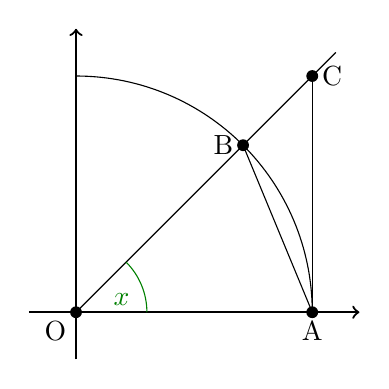
\begin{tikzpicture}[scale=3]
		\draw[->, thick] (-0.2,0) -- (1.2,0);
		\draw[->, thick] (0,-0.2) -- (0,1.2);

		\draw (1,0) arc [radius=1, start angle=0, end angle=90];
		\draw (0,0) -- (1.1, 1.1);

		\draw[green!50!black] (0.3, 0) arc [radius=0.3, start angle=0, end angle=45];
		\draw[green!50!black] (15:0.2) node{$x$};

		\draw (1, 0) -- ({cos(45)}, {sin(45)});
		\fill (1, 0) circle (0.025) node[anchor=north]{A};
		\fill ({cos(45)}, {sin(45)}) circle (0.025) node[anchor=east]{B};
		\fill (0, 0) circle (0.025) node[anchor=north east]{O};
		\draw (1, 0) -- (1, 1);
		\fill (1, 1) circle (0.025) node[anchor=west]{C};
	\end{tikzpicture}
\end{figure}

\section{Непрерывность функции в точке; арифметические свойства \texorpdfstring{\\}{} непрерывных в точке функций}

\begin{definition}
	$X, \rho, \quad A$ -- т. сг., $\quad A \in X, \quad f : X \to \R$
	$$ f \text{ непрерывна в } A \iff \exist \liml{x \to A} f(x) = f(A) $$
	Что эквивалентно:
	$$ \forall \veps > 0 ~ \exist \delta > 0 : \forall x \in X \quad \rho(x, A) < \delta \implies |f(x) - f(A)| < \veps $$
	Или:
	$$ \forall \omega(f(A)) ~ \exist \Omega(A) : \forall x \in \Omega(A) \quad f(x) \in \omega(f(A)) $$
\end{definition}

\begin{properties}
	\hfill
	\begin{enumerate}
		\item $f(x) \equiv C \implies f $ непр. в $A$
		\item $f$ непр. в $A \implies cf $ непр. в $A$
		\item $f, g$ непр. в $A \implies f + g$ непр. в $A$
		\item $f, g$ непр. в $A \implies f \cdot g $ непр. в $A$
		\item $
		\begin{rcases}
			f \text{ непр. в } A \\
			\forall x \in X \quad f(x) \ne 0
		\end{rcases} \implies \dfrac1f \text{ непр. в } A$
		\begin{proof}
			$ \liml{x \to A} = f(A) \ne 0 \implies \liml{x \to A}\dfrac1{f(x)} = \liml{x \to A}\dfrac1{f(A)} \ne 0$
		\end{proof}
		\item $
		\begin{rcases}
			f \text{ как в 5 пункте} \\
			g \text{ непр. в } A
		\end{rcases} \implies \dfrac{g}f \text{ непр. в } A$
	\end{enumerate}
\end{properties}

\section{Непрерывность суперпозиции непрерывных в точках \texorpdfstring{\\}{} функций}

\begin{property}
	$E \sub \R, \quad a \in E$ -- т. сг. $E$ \\
	$F \sub \R, \quad b \in F$ -- т. сг. $F$ \\
	$f: E \to F, \quad f(a) = b$ \\
	$ g : F \to \R $ \\
	$ h(x) = g(f(x)), \quad h : E \to \R $
	$$ \begin{rcases}
		f(x) \text{ непр. в } a \\
		g(y) \text{ непр. в } b
	\end{rcases} \implies h \text{ непр. в } a $$
\end{property}

\begin{proof}
	$$ h(a) \bydef g(f(a)) \bydef g(b) \implies \forall \omega(h(a)) = \omega(g(b)) $$
	\begin{equ}{431}
		g \text{ непр. в } b \iff \exist \Omega(b) : \forall y \in \Omega(b) \cap F \quad g(y) \in \omega(g(b))
	\end{equ}
	$$ b = f(a) \implies \Omega(b) = \Omega(f(a)) $$
	\begin{equ}{432}
		f \text{ непр. в } a \iff \exist \Lambda(a) : \forall x \in E \cap \Lambda(a) \quad f(x) \in \Omega(f(a))
	\end{equ}
	Возьмём $\forall x \in E \cap \Lambda(a)$
	$$ \eref{432} \implies f(x) \in \Omega(f(a)) \cap F = \Omega(b) \cap F $$
	То есть, можно применить \eref{431}
	$$ \eref{431} \implies g(f(x)) \in \omega(g(b)) = \omega(h(a)) \implies h(x) \in \omega(h(a)) $$
\end{proof}

\section({Непрерывность p(x), p(x)/q(x), e\text{\textasciicircum}x}){Непрерывность $\bm{p(x)}$, $\bm{\frac{p(x)}{q(x)}}$, $\bm{e^x}$}

\begin{property}
	$p(x) = c_0 + c_1x + ... + c_nx^n$ \\
	$ p(x) \in C(\R) $

\end{property}

\begin{property}
	$q(x) = b_0 + b_1x + ... + b_tx^t $ \\
	$a_1, ..., a_n$ -- все числа : $p(a_k) = 0$
	$$ \frac{q(x)}{p(x)} \in C(\R \setminus {a_1, ..., a_n}) $$
\end{property}

\begin{property}
	$e^x \in C(\R)$
\end{property}

\begin{proof}
	$$ e^h \underarr{h \to 0} 1 $$
	$$ \forall x_0 \ne 0
	\begin{Bmatrix}
		\quad e^x = x^{x_0} \cdot e^{x - x_0} \\
		x - x_0 \in C(\R)
	\end{Bmatrix} \underimp{\text{как суперпозиция}} e^x \text{ непр. в } x_0 \underimp{\text{в силу произв. } x_0} e^x \in C(\R) $$
\end{proof}

\section({Непрерывность ln x, x\text{\textasciicircum}r}){Непрерывность $\bm{\ln x}$, $\bm{x^r}$}

\begin{replacementproof}[непрервыность $\ln x$]
	$$ \ln (1 + h) \underarr{h \to 0} \ln 1 $$
	$$ \ln (1 + h) = \frac{\ln(1 + h)}h \cdot h \implies \ln(x) \text{ непр. в } 1 $$
	Возьмём $x_0 >0, \quad x_0 \ne 1$
	$$ \ln x = \ln x \cdot \frac{x}{x_0} + \ln x_0 \implies \ln x \text{ непр. в } x_0 $$
	$$ \frac{x}{x_0} \in C(\R), \quad \frac{x_0}x = 1 \implies \ln x \in C(0, +\infty) $$
\end{replacementproof}

\begin{replacementproof}[непрерывность $x^r$]
	$$ x > 0, r \in \R \implies x^r \in C(0, +\infty) $$
	$$ r > 0, \quad 0^r \bydef 0 \implies x^r \text{ непр. в } 0 $$
	$x^r$ монотонно возрастает при $x > 0$ \\
	Возьмём $\delta : \forall \veps > 0 \quad \delta^r = \veps, \quad \delta = \veps^{1/\delta} $ \\
	При $x < \delta \quad 0 < x^r < \delta^r = (\veps^{1/r})^r = \veps $
\end{replacementproof}

\section{Теорема об обращении непрерывной функции в ноль}

\begin{theorem}
	$$ f \in C([a,b]) $$
	\begin{equ}{461}
		f(a) \cdot f(b) < 0
	\end{equ}
	$$ \implies \exist c \in [a,b] : f(c) = 0 $$
\end{theorem}

\begin{proof}
	Будем определять вложенные промежутки $[a_n, b_n]$
	$$ a_1 \define a, \quad b_1 \define b $$
	$$ \eref{461} \iff f(a_1) \cdot f(b_1) < 0 $$
	$$ c_1 \define \frac{a_1 + b_2}2 = \frac{a + b}2 $$
	\begin{itemize}
		\item Если $f(c_1) = 0$, то $c \define c_1$
		\item Иначе:
		$$ \eref{461} \implies \left[
		\begin{aligned}
			f(a_1) \cdot f(c_1) < 0 \\
			f(c_1) \cdot f(b_1) < 0
		\end{aligned} \right. $$
		$ [a_2, b_2] $ -- тот из $[a_1, c_1], [c_1, b_1] $, для которого $ f(a_2) \cdot f(b_2) < 0 $
		$$ c_2 \define \frac{a_2 + b_2}2 $$
		\begin{itemize}
			\item Если $f(c_2) = 0$, то $c \define c_2$
			\item Иначе:
			$$ \eref{461} \implies \left[
			\begin{aligned}
				f(a_2) \cdot f(c_2) < 0 \\
				f(c_2) \cdot f(b_2) < 0
			\end{aligned} \right. $$
			$[a_3, b_3]$ -- тот из $[a_2, c_2], [c_2, b_2] $, для которого $ f(a_3) \cdot f(b_3) < 0 $
			$$ \widedots $$
			$[a_n, b_n]$ -- тот из $[a_{n - 1}, c_{n - 1}], [c_{n - 1}, b_{n - 1}]$, для которого $ f(a_n) \cdot f(b_n) < 0 $
			$$ c_n \define \frac{a_n + b_n}2 $$
			\begin{itemize}
				\item Если $f(c_n) = 0$, то $c \define c_n$
				\item Иначе:
				$$ \eref{461} \implies \left[
				\begin{aligned}
					f(a_n) \cdot f(c_n) < 0 \\
					f(c_n) \cdot f(b_n) < 0
				\end{aligned} \right. $$
				Индукционный переход: $[a_{n + 1}, b_{n + 1}]$ -- тот из $[a_n, c_n]$, для которого $f(a_{n + 1}) \cdot f(b_{n + 1}) < 0 $ \\
				Пусть такое $n$ не нашлось, то есть:
				$$ \forall n
				\begin{cases}
					c_n = \dfrac{a_{n + 1}, b_{n + 1}}2 \\
					f(c_n) \ne 0 \\
					f(a_n) \cdot f(b_n) < 0
				\end{cases} $$
				Тогда, по построению:
				$$ \begin{rcases}
					b_n - a_n = \dfrac{b - a}{2^{n - 1}} \underarr{x \to \infty} 0 \\
					\forall n \quad [a_{n + 1}, b_{n + 1}] \supset [a_n, b_n]
				\end{rcases} \implies \forall n ~ \exist c \in [a_n, b_n] \text{ (по т. о вложенных промежутках)} $$
				\begin{equ}{463}
					\left.
					\begin{aligned}
						a_n \to c \\
						b_n \to c \\
						f \in C([a, b]) \implies f \text{ непр. в } c
					\end{aligned} \right\} \implies
					\begin{Bmatrix}
						f(a_n) \to f(c) \\
						f(b_n) \to f(c)
					\end{Bmatrix} \implies f(a_n) \cdot f(b_n) \to f^2(c)
				\end{equ}
				$$ f(a_n) \cdot f(b_n) < 0 \implies \limz{n} (f(a_n) \cdot f(b_n)) \le 0 \underimp{\eref{463}} f^2(c) \le 0 \implies f(c) = 0 $$
			\end{itemize}
		\end{itemize}
	\end{itemize}
\end{proof}

\section{Теорема о промежуточном значении непрерывной функции}

\begin{theorem}
	$ f \in C([a,b]), \quad f(a) = p, \quad f(b) = q, \quad p \ne q $
	\begin{equ}{471}
		\min(p, q) < r < \max(p, q) \implies \exist c \in (a, b) : f(c) = r
	\end{equ}
\end{theorem}

\begin{proof}
	Возьмём $g(x) = f(x) - r$
	\begin{multline*}
		g(a) \cdot g(b) = (f(a) - r) \cdot (f(b) - r) = (p - q)(q - r) < 0 \underimp{\text{по т. об обр. непр. функции в ноль}} \\ \implies \exist c \in (a, b) : g(c) = 0
	\end{multline*}
	$$ f(c) - r = 0 \implies \eref{471}$$
\end{proof}

\section{Классификация точек разрыва; точки разрыва монотонной \texorpdfstring{\\}{} функции}

\begin{statement}
	$E \sub \R, \quad a \in E, \quad a$ -- т. сг. $E$ \\
	$f : E \to \R, \quad f$ не непр. в $a$ -- т. разрыва
	\begin{enumerate}
		\item Устранимая точка разрыва: \\
		$a \in (p, q), \quad f : (p, q) \to \R $ \\
		$\begin{cases}
		 	\exist \liml{x \to a-0} f(x) \in \R \\
			\exist \liml{x \to a - 0} f(x) \in \R
		 \end{cases}$ \\
		 $\liml{x \to a-0} f(x) = \liml{x \to a + 0} f(x) \ne f(a) \iff a$ -- устранимая точка разрыва
		 \item Разрыв \rom1 рода (скачок)
		 \begin{enumerate}
		 	\item $a \in (p, q)$ \\
			$ \begin{cases}
				\exist \liml{x \to a-0} f(x) \in \R \\
				\exist \liml{x \to a +0} f(x) \in \R \\
				\liml{x \to a -0} f(x) \ne \liml{x \to a +0} f(x)
			  \end{cases} $
			  \item $f: [a, q) \to \R, \quad \exist \liml{x \to a + 0} f(x) \ne f(a) $
			  \item $f : (p, a] \to \R, \quad \exist \liml{x \to a -0} f(x) \ne f(a) $
		 \end{enumerate}
		\item Разрыв \rom2 рода \\
		По крайней мере $\liml{x \to a-0} f(x) $ или $\liml{x \to a + 0} f(x)$ не существует или бесконечен
	\end{enumerate}
\end{statement}

\begin{theorem}[о множестве разрывов монотонной функции]
	$$ f : [a, b] \text{ -- монотонна } \implies \forall x_0 \in [a, b] \left[
	\begin{tabular}{l}
		$f$ непрерывна в $ x_0 $ \\
		$f$ имеет разрыв \rom1 рода в $ x_0 $
	\end{tabular} \right. $$
\end{theorem}

\begin{replacementproof}[для возрастающей]
	Рассмотрим случай, когда $x_0 \in (a, b)$ \\
	Применим теорему о пределе монотонной функции:
	$$ \begin{rcases}
		\forall x \in (a, x_0) \quad f(x) \le f(x_0) \implies \exist \liml{x \to x_0 - 0} f(x) \le f(x_0) \\
		\forall x \in (x_0, b) \quad f(x_0) \le f(x) \implies \exist \liml{x \to x_0+0} f(x) \ge f(x_0)
	\end{rcases} \iff \liml{x \to x_0 - 0} f(x) \le f(x_0) \le \liml{x \to x_0+0} f(x) $$
	Значит:
	\begin{itemize}
		\item Либо все эти три значения равны, и $f$ непрерывна в $x_0$
		\item Либо $\liml{x \to x_0-0} f(x) < \liml{x \to x_0 + 0} f(x)$, и $x_0$ -- разрыв \rom1 рода
	\end{itemize}
\end{replacementproof}

\section{Теорема об отображении отрезка}

\begin{theorem}
	$f : [a, b], \quad f$ монотонна, $\quad f(a) = p, \quad f(b) = q, \quad p \ne q $
	$$ f([a,b]) = [\min(p, q), \max(p, q)] \iff f \in C([a,b]) $$
\end{theorem}

\begin{proof}
	\hfill
	\begin{itemize}
		\item $\impliedby$ \\
		Возьмём $\forall r \in [\min(p, q), \max(p, q)] $ \\
		По теореме о промежуточном значении непрерывной функции, $ \exist c \in (a, b) : f(c) = r $ \\
		В силу прозвольности $r$:
		\begin{equ}{4923}
			f([a, b]) \supset [\min(p, q), \max(p, q)]
		\end{equ}
		Поскольку $f$ монотонна,
		$$ \forall x \in [a, b] \quad f(x) \in [\min(p, q), \max(p, q)] $$
		То есть
		$$ f([a, b]) \sub [\min(p, q), \max(p, q)] \underimp{\eref{4923}} f([a, b]) = [\min(p, q), \max(p, q)] $$
		\item $\implies$
		\begin{equ}{4924}
			f([a, b]) = [\min(p, q), \max(p, q)]
		\end{equ}
		Предположим, что $f \notin C([a, b])$ \\
		По определению, это означает, что $ \exist x_0 \in [a, b] : f $ разрывна в $ x_0 $ \\
		Рассмотрим случай, когда $x_0 \in (a, b)$ и $f$ возрастает \\
		По теореме о множестве разрывов монотонной функции, $x_0$ -- разрыв \rom1 рода, то есть
		$$ \liml{x \to x_0-0}f(x) = A < B = \liml{x \to x_0+0}f(x) $$
		Рассмотрим
		\begin{equ}{4927}
			y_0 \in (A, B), \quad y_0 \ne f(x_0)
		\end{equ}
		По теореме о пределе монотонной функции, имеем следующие соотношения:
		$$ \left.
		\begin{aligned}
			\begin{rcases}
				\forall x < x_0 \quad f(x) \le A \\
				\forall x > x_0 \quad f(x) \ge B
			\end{rcases} \underimp{\eref{4927}} \forall \underset{x \ne x_0}{x \in [a,b]} \quad f(x) \ne y_0 \\
			\eref{4927} \implies f(x_0) \ne y_0
		\end{aligned} \right\} \implies y_0 \notin f([a, b]) \quad \contra \eref{4924} $$
		Значит, наше предположение неверно, и $f \in C([a, b])$
	\end{itemize}
\end{proof}


\section{Существование и непрерывность обратной функции}

\begin{theorem}
	$f \in C([a, b]), \quad f $ строго монотонна, $ \quad [p, q] = f([a, b]) $
	$$ \implies \exist g : [p, q] \to \R : g \in C([p, q]) $$
	\begin{equ}{502}
		\begin{cases}
			\forall x \in [a, b] \quad g(f(x)) = x \\
			\forall y \in [p, q] \quad f(g(y)) = y
		\end{cases}
	\end{equ}

	\begin{itemize}
		\item Если $f$ возрастает, то $g$ возрастает
		\item Если $f$ убывает, то $g$ убывает
	\end{itemize}
\end{theorem}

\begin{replacementproof}[для возрастающей]
	\begin{equ}{505}
		\forall y \in (p, q) \quad \exist x \in (a, b) : f(x) = y
	\end{equ}
	$f$ строго возрастает, значит
	\begin{equ}{506}
		\begin{rcases}
			x_1 < x \implies f(x_1) < f(x) = y \\
			x_2 > x \implies f(x_2) > f(x) = y
		\end{rcases}
	\end{equ}
	$$ \eref{505}, \eref{506} \implies \forall y ~ \exist! x : f(x) = y $$
	\begin{equ}{508}
		\text{Определим } g: \text{ полагагаем } g(y) \define x, \quad f(x) \define y
	\end{equ}
	$$ \eref{508} \implies \eref{502} $$
	Мы доказали, что у функции $f$ есть обратная \\
	Проверим её непрерывность и монотонность:
	\begin{itemize}
		\ \item Монотонность: \\
		Возьмём $y_1 < y_2 \in [p, q]$ \\
		Обозначим $x_1 \define g(y_1), \quad x_2 \define g(y_2)$ \\
		Очевидно, что $x_1 \ne x_2$ (в силу \eref{508}). Остаётся $x_1 < x_2$ или $x_1 > x_2$ \\
		Допустим, $x_1 > x_2 \implies f(x_1) = y_1 > y_2 = f(x_2) $ -- \contra с \eref{506} \\
		Тогда $ x_1 < x_2 \implies g(y) $ строго возрастает
		\item Непрерывность: \\
		Очевидно, что $g([p, q]) \sub [a, b]$ (в силу \eref{508}) \\
		Возьмём $\forall x_0 \in [a, b]$ \\
		Пусть $y_0 \define f(x_0)$. Очевидно, что $y_0 \in [p, q]$
		$$ \eref{508} \implies g(y_0) = x_0 \implies g([p, q]) = [a, b] $$
		Применим теорему об отображении отрезка: $g$ отображает $[p, q]$ на $[a, b]$ и $g$ строго монотонна, значит, $g$ непрерывна
	\end{itemize}
\end{replacementproof}

\section({Непрерывность sin x, cos x, tg x, ctg x}){Непрерывность $\bm{\sin x}$, $\bm{\cos x}$, $\bm{\tg x}$, $\bm{\ctg x}$}

\begin{statement}
	$\sin x \in C(\R), \quad \cos x \in C(\R)$
\end{statement}

\begin{proof}
	Нужно доказать, что $\sin x$ непрерывна при $x = x_0$ и $\cos x$ непрерывна при $x = x_0$. Рассмотрим два случая:
	\begin{itemize}
		\item $x_0 = 0$
		\begin{itemize}
			\item $\sin x$
			$$ \sin x = \underbrace{\frac{\sin x}x}_{\to 1} \cdot \underbrace{x}_{\to 0} \underarr{x \to 0} 0, \quad \sin 0 = 0 $$
			\item $\cos x$ \\
			Воспользуемся правилом двух милиционеров:
			$$ 1 - |x| \le \sqrt{1 - x^2} \le \cos x = \sqrt{1 - \sin^2 x} \le 1 \implies \cos x \underarr{x \to 0} 0, \quad \cos 0 = 1 $$
		\end{itemize}
		\item $x_0 \ne 0$
		\begin{itemize}
			\item $\sin x$
			$$ \sin x = \sin ((x - x_0) + x_0) = \sin(\underbrace{x - x_0}_{\in C(\R)}) \cdot \underbrace{\cos x_0}_{\text{const}} + \cos (\underbrace{x - x_0}_{\in C(\R)}) \cdot \underbrace{\sin x_0}_{\text{const}} $$
			Мы уже доказали, что $\sin x$, $\cos x$ непрерывны в $0$ \\
			Если $x - x_0 = 0$, то $\sin (x - x_0) = 0$ \\
			По теореме о суперпозиции непрерывных функций, $\sin x$ непрерывна при $x = x_0 \ne 0$
			\item $\cos x$
			$$ \cos x = \cos ((x - x_0) + x_0) = \cos (x - x_0) \cdot \cos x_0 - \sin (x - x_0) \cdot \sin x_0 $$
			Аналогично получаем, что $\cos x$ непрерывна при $x = x_0 \ne 0$
		\end{itemize}
	\end{itemize}
	$$ \implies \sin x, \cos x \in C(\R) $$
\end{proof}

\begin{statement}
	$ \tg x \in C(\R \setminus \set{\frac{\pi}2 + \pi n, n \in \Z}) $
\end{statement}

\begin{proof}
	$$ \tg x = \frac{\sin x}{\cos x} $$
	При $x \ne \frac{\pi}2 + \pi n, n \in Z$, знаменатель не обращается в ноль, а, значит, можно применить свойство о частном непрерывных функций
\end{proof}

\begin{statement}
	$ \ctg x \in C(\R \setminus \set{\pi n, n \in Z}) $
\end{statement}

\begin{proof}
	$$ \ctg x = \frac{\sin x}{\cos x} $$
	Дальше рассуждение аналогичное
\end{proof}

\section({Непрерывность arcsin x, arccos x}){Непрерывность $\bm{\arcsin x}$, $\bm{\arccos x}$}

\begin{statement}
	$ \arcsin x, \arccos x \in C([-1, 1]) $
\end{statement}

\begin{proof}
	Рассмотрим $\sin x \clamp{[-\frac{\pi}2, \frac{\pi}2]} $. Она строго возрастает \\
	$\sin (-\frac{\pi}2) = 1, \quad \sin(\frac{\pi}2) = 1$ \\
	Значит, в силу теоремы об обратной функции, у неё есть обратная функция $\arcsin y, \quad y \in [-1, 1] $, которая тоже строго возрастает и непрерывна \\
	Рассмотрим $\cos x \clamp{[0, \pi]} $. Она строго убывает \\
	Аналогично, существует и непрерывна $\arccos y, \quad y \in [-1, 1] $
\end{proof}

\section({Непрерывность arctg x, arcctg x}){Непрерывность $\bm{\arctg x}$, $\bm{\arcctg x}$}

\begin{statement}
	$\arctg x \in C(\R)$
\end{statement}

\begin{proof}
	Обозначим $a_n \define -\frac{\pi}2 + \frac{\pi}{4n}, \quad b_n \define \frac{\pi}2 - \frac{\pi}{4n}, \quad p_n \define \tg a_n, \quad q_n \define \tg b_n $ \\
	Заметим, что
	$$ \begin{cases}
		[a_n, b_n] \sub [a_{n + 1}, b_{n + 1}] \\
		[p_n, q_n] \sub [p_{n + 1}, q_{n + 1}]
	\end{cases} $$
	Рассмотрим $\tg x \clamp{[a_n, b_n]}$. Она строго возрастает \\
	Значит, по теореме об обратной функции, на $[p_n, q_n]$ существует и непрерывна $\arctg y$ \\
	По построению промежутков,
	$$ \arctg x \in C(\bigcup_{n = 1}^\infty [p_n, q_n]) $$
	Несложно заметить, что
	$$ \begin{rcases}
	   	p_n \underarr{n \to \infty} -\infty \\
		q_n \underarr{n \to \infty} +\infty
	\end{rcases} \implies \bigcup_{n = 1}^\infty[p_n, q_n] = \R \implies \arctg x \in C(\R) $$
\end{proof}

\begin{statement}
	$\arcctg x \in C(\R)$
\end{statement}

\begin{proof}
	Доказательство аналогичное
\end{proof}

\section{Первая теорема Вейерштрасса}

\begin{theorem}
	$ f \in C([a, b]) \implies \exist M, L : \forall x \in [a, b] \quad L \le f(x) \le M $
\end{theorem}

\begin{proof}
	Пусть $ \not\exist M : \forall x \in [a, b] \quad f(x) \le M $ \\
	Тогда:
	\begin{equ}{543}
		\begin{rcases}
			\exist x_1 \in [a, b] : f(x_1) > 1 \\
			\exist x_2 \in [a, b] : f(x_2) > f(x_1) + 2 \\
			\widedots \\
			\exist x_n \in [a, b] : f(x_n) > f(x_{n - 1}) + n
		\end{rcases}
	\end{equ}
	$$ \eref{543} \implies f(x_n) \underarr{n \to \infty} +\infty $$
	\begin{equ}{545}
		x_n \in [a, b]
	\end{equ}
	Применим принцип выбора Больцано-Вейерштрасса:
	\begin{equ}{546}
		\eref{545} \iff \seq{x_n}n \text{ ограничена} \implies
		\begin{Bmatrix}
			\exist x_* \in [a, b] \\
			\exist \seq{x_k}k
		\end{Bmatrix} : x_{n_k} \underarr{k \to \infty} x_*
	\end{equ}
	\begin{equ}{547}
		f \in C([a, b]) \iff f \text{ непрерывна в каждой точке } [a, b] \text{, в частности } f \text{ непрерывна в } x_*
	\end{equ}
	По теореме о связи пределов последовательностей с переделом функции:
	$$ \eref{546}, \eref{547} \implies f(x_{n_k}) \underarr{k \to \infty} f(x_*) \in \R $$
	\begin{equ}{549'}
		\text{Это означает, что она ограничена, то есть } \exist A : \forall k \quad |f(x_{n_k})| \le A
	\end{equ}
	\begin{equ}{5410}
		\eref{543} \implies f(x_{n_k}) > n_k \ge k
	\end{equ}
	$$ \eref{549'}, \eref{5410} \implies \forall k \quad k < A \text{ -- \contra (т. к. } k \text{ должно пробегать весь натуральный ряд)} $$
	Для $L$ доказывается точно так же
\end{proof}

\section{Вторая теорема Вейерштрасса}

\begin{theorem}
	$f \in C([a, b]) \implies
	\begin{Bmatrix}
		\exist x_- \in [a, b] \\
		\exist x_+ \in [a, b]
	\end{Bmatrix} : \forall x \in [a, b] \quad f(x_-) \le f(x) \le f(x_+) $
\end{theorem}

\begin{proof}
	Пусть $ \not\exist x_+ \in [a, b] : \forall x \in [a, b] \quad f(x) \le f(x_+) $ \\
	Рассмотрим $E = f([a, b])$ \\
	По первой теореме Вейерштрасса, $ \exist M : \forall x \in [a, b] \quad f(x) \le M \implies E $ ограничено сверху \\
	Это значит, что у него есть супремум. Обозначим его
	\begin{equ}{5513}
		y_0 \define \sup E
	\end{equ}
	$$ \eref{5513} \implies \forall x \in [a, b] \quad f(x) \le y_0 $$
	Если бы $\exist x_+$, то $ f(x_+) = y_0 $. Однако, мы предположили, что $\not\exist x_+$. Значит, $ f(x_+) \ne y_0 $ и:
	\begin{equ}{5515}
		\forall x \in [a, b] \quad f(x) < y_0
	\end{equ}
	Рассмотрим $\vphi(x) \define y_0 - f(x)$
	$$ \begin{rcases}
		\eref{5515} \implies \forall x \in [a, b] \quad \vphi(x) > 0 \\
		\vphi \bydef[\in] C([a, b])
	\end{rcases} \implies \frac1\vphi \in C([a,b]) $$
	Тогда можно применить к $\frac1\vphi$ первую теорему Вейерштрасса:
	\begin{multline*}
		\forall x \in [a, b] \quad \exist Q : \frac1{\vphi(x)} \le Q \iff \frac1Q \le y_0 - f(x) \iff f(x) \le y_0 - \frac1Q \iff \\ \iff y_0 - \frac1Q \text{ -- верхняя граница } E \contra \eref{5513}
	\end{multline*}
\end{proof}

\section{Теорема Кантора}

\begin{theorem}
	$f \in C([a, b]) \implies f $ равномерно непрерывна на $[a, b]$
\end{theorem}

\begin{proof}
	Пусть $f$ не равномерно непрерывна на $[a, b]$, то есть
	\begin{equ}{5624}
		\exist \veps_0 : \forall \delta > 0 ~ \exist x_{1\delta}, x_{2\delta} \in [a, b] :
		\begin{cases}
			|x_{2\delta} - x_{1\delta}| < \delta \\
			|f(x_{2\delta}) - f(x_{1\delta})| \ge \veps_0
		\end{cases}
	\end{equ}
	Возьмём $\delta_n \define \frac1n, \quad x_{1n}' \define x_{1, \faktor1n}, \quad x_{2n}' \define x_{2, \faktor1n} $
	\begin{equ}{5625}
		\eref{5624} \implies
		\begin{cases}
			|x_{2n}' - x_{1n}'| < \frac1n \\
			|f(x_{2n}') - f(x_{1n}')| \ge \veps_0
		\end{cases}
	\end{equ}
	$\forall n \quad x_{1n}' \bydef[\in] [a, b] $, значит к ней можно применить принцип выбора Больцано-Вейерштрасса:
	\begin{equ}{5626}
		\exist
		\begin{Bmatrix}
			x_* \in [a, b] \\
			\seq{x_{1n_k}'}k
		\end{Bmatrix} : x_{1n_k}' \underarr{k \to \infty} x_*
	\end{equ}
	Определим $y_n \define x_{2n}' - x_{1n}'$
	\begin{equ}{5628}
		\eref{5625} \implies y_n \underarr{n \to \infty} 0 \implies y_{n_k} \underarr{x \to \infty} 0 \underimp{\eref{5626}} x_{2n_k}' = x_{1n_k}' + y_{n_k} \underarr{k \to \infty} x_*
	\end{equ}
	\begin{equ}{5629}
		f \in C([a, b]) \text{, в частности, } f \text{ непрерывна в } x_*
	\end{equ}
	Применим теорему о связи пределов последовательностей с пределом функции:
	\begin{equ}{5630}
		\eref{5626}, \eref{5628}, \eref{5629} \implies
		\begin{Bmatrix}
			f(x_{1n_k}') \underarr{k \to \infty} f(x_*) \\
			f(x_{2n_k}') \underarr{k \to \infty} f(x_*)
		\end{Bmatrix} \iff
		\begin{cases}
			\exist N_1 : \forall k > N_1 \quad |f(x_{1n_k}') - f(x_*)| < \veps \\
			\exist N_2 : \forall k > N_2 \quad |f(x_{2n_k}') - f(x_*)| < \veps
		\end{cases}
	\end{equ}
	Возьмём $k_0 \definerel> N_1 + N_2$. Тогда
	\begin{equ}{5633}
		|f(x_{2n_{k_0}}') - f(x_{1n_{k_0}}')| \underset{\text{нер-во } \vartriangle}\le |f(x_{2n_{k_0}}') - f(x_*) | + |f(x_*) - f(x_{1n_{k_0}}')| \underset{\eref{5630}}< \veps + \veps = \veps
	\end{equ}
	Вспомним, что, по \eref{5625}, $|f(x_{2n}') - f(x_{1n}')| \ge \veps_0$. В частности,
	\begin{equ}{5634}
		|f(x_{2n_{k_0}}') - f(x_{2n_{k_0}}')| \ge \veps_0
	\end{equ}
	Возьмём $\veps \define \dfrac{\veps_0}2$. Тогда
	$$ \eref{5633} \implies |f(x_{2n_{k_0}}') - f(x_{1n_{k_0}}')| < \veps_0 \text{ -- \contra \eref{5634}} $$
\end{proof}

\section{Определение производной; дифференцируемости}

\begin{definition}
	\hfill
	\begin{itemize}
		\item $f : (a, b) \to \R, \quad x_0 \in (a, b)$
		$$ f \text{ имеет производную в } x_0 \iff \exist \limz{h} \frac{f(x_0 + h) - f(x_0)}h \in \R $$
		\item $f : [a, b) \to \R $
		$$ f \text{ имеет правую производную в } a \iff \exist \liml{h \to +0} \frac{f(a + h) - f(a)}h \in \R $$
		\item $f : (a, b] \to \R $
		$$ f \text{ имеет левую производную в } b \iff \exist \liml{h \to -0} \frac{f(b + h) - f(b)}h \in \R $$
	\end{itemize}
\end{definition}

\begin{definition}
	$f : (a, b) \to \R, \quad x_0 \in (a, b) $
	$$ f \text{ дифференцируема в } x_0 \iff \exist
	\begin{Bmatrix}
		A \in \R \\
		r : (a, b) \to \R
	\end{Bmatrix} :
	\begin{cases}
		f(x) - f(x_0) = A(x - x_0) + r(x) \\
		\frac{r(x)}{x - x_0} \underarr{x \to x_0} 0
	\end{cases} $$
\end{definition}

\begin{note}
	Определение дифференцируемости можно переписать так:
	$$ f \text{ дифференцируема в } x_0 \iff \exist
	\begin{Bmatrix}
		A \in \R \\
		\omega(0) \\
		\rho(h) : \omega(0) \to \R
	\end{Bmatrix} :
	\begin{cases}
		f(x_0 + h) - f(x_0) = Ah + \rho(h) \\
		\frac{\rho(h)}h \underarr{h \to 0} 0
	\end{cases} $$
\end{note}

\section{Теорема о связи производной и дифференцируемости}

\begin{theorem}
	$f$ дифференцируема в $x_0 \iff \exist f'(x_0)$ \\
	При этом, для $A$ из определения дифференцируемости имеем $A = f'(x_0)$
\end{theorem}

\begin{proof}
	\hfill
	\begin{itemize}
		\item $\impliedby$ \\
		Пусть $\exist f'(x_0)$. Это значит, что
		\begin{equ}{5811}
			\delta(h) \define \frac{f(x_0 + h) - f(x_0)}h - f'(x_0) \underarr{x \to 0} 0
		\end{equ}
		\begin{equ}{5812}
			\text{Положим }\rho(h) \define h\delta(h)
		\end{equ}
		Умножим \eref{5811} на $h$:
		\begin{equ}{5813}
			\eref{5811}, \eref{5812} \implies f(x_0 + h) - f(x_0) - f'(x_0)h = h\delta(h) = \rho(h)
		\end{equ}
		\begin{equ}{5914}
			\eref{5813} \iff f(x_0 + h) - f(x_0) = f'(x_0)h + \rho(h), \quad \frac{\rho(h)}h = \delta(h) \underarr{h \to 0} 0
		\end{equ}
		Можно взять $A \define f'(x_0)$
		\item $\implies$ \\
		Пусть $f$ дифференцируема в $x_0$. Тогда, по ``альтернативному'' определению дифференцируемости,
		$$ f(x_0 + h) - f(x_0) = Ah + \rho(h) \iff \frac{f(x_0 + h) - f(x_0)}h = A + \frac{\rho(h)}h \xrightarrow[h \to 0]{\text{def}} A \in \R $$
		То есть, $\exist f'(x_0) = A$
	\end{itemize}
\end{proof}

\section({Свойства производных для cf(x), f(x) + g(x), f(x)g(x)}){Свойства производных для $\bm{cf(x)}$, $\bm{f(x) + g(x)}$, $\bm{f(x)g(x)}$}

\begin{properties}
	$f, g: (a, b) \to \R, \quad x_0 \in (a, b), \quad f, g$ диффернцируемы в $x_0$
	\begin{enumerate}
		\item $(cf)'(x_0) = cf'(x_0)$
		\begin{proof}
			$$ \frac{cf(x_0 + h) - cf(x_0)}h = c \cdot \frac{f(x_0 + h) - f(x_0)}h \underarr{h \to 0} cf'(x_0) $$
		\end{proof}
		\item $(f + g)'(x_0) = f'(x_0) + g'(x_0) $
		\begin{proof}
			\begin{multline*}
				\frac{f(x_0 + h) + g(x_0 + h) - f(x_0) - g(x_0)}h = \frac{f(x_0 + h) - f(x_0)}h + \frac{g(x_0 + h) - g(x_0)}h \underarr{h \to 0} \\ \to f'(x_0) + g'(x_0)
			\end{multline*}
		\end{proof}
		\item $(fg)'(x_0) = f'(x_0)g(x_0) + f(x_0)g'(x_0) $
		\begin{proof}
			\begin{multline*}
				\frac{f(x_0 + h)g(x_0 + h) - f(x_0)g(x_0)}h = \\ = \frac{f(x_0 + h)g(x_0 + h) - f(x_0)g(x_0 + h) + f(x_0)g(x_0 + h) - f(x_0)g(x_0)}h = \\ = \frac{\bigg( f(x_0 + h) - f(x_0) \bigg) \cdot g(x_0 + h)}h + \frac{f(x_0) \cdot \bigg( g(x_0 + h) - g(x_0) \bigg)}h \underarr{h \to 0} \\ \to f'(x_0)g(x_0) + f(x_0)g'(x_0)
			\end{multline*}
		\end{proof}
	\end{enumerate}
\end{properties}

\section({Свйоства производных для 1/f(x), g(x)/f(x)}){Свойства производных для $\bm{\frac1{f(x)}}$, $\bm{\frac{g(x)}{f(x)}}$}

\begin{properties}
	$f(x) \ne 0$ при $x \in (a, b)$
	\begin{enumerate}
		\item $(\faktor1f)'(x_0) = - \dfrac{f'(x_0)}{f^2(x_0)}$
		\begin{proof}
			\begin{multline*}
				\frac{\dfrac1{f(x_0 + h)} - \dfrac1{f(x_0)}}h = \frac{\dfrac{f(x_0) - f(x_0 + h)}{f(x_0 + h)f(x_0)}}h = \\ = - \frac1{f(x_0)} \cdot \frac1{f(x_0 + h)} \cdot \frac{f(x_0 + h) - f(x_0)}h \underarr{h \to 0} -\frac{f'(x_0)}{f^2(x_0)}
			\end{multline*}
		\end{proof}
		\item $(\faktor{g}f)'(x_0) = \dfrac{g'(x_0)f(x_0) - g(x_0)f'(x_0)}{f^2(x_0)}$
		\begin{proof}
			Используем свойства о произведении и $\faktor1f$:
			\begin{multline*}
				(\faktor{g}f)'(x_0) = \bigg( g \cdot \frac1f \bigg)'(x_0) = g'(x_0) \cdot \frac1{f(x_0)} + g(x_0) \cdot \bigg(\frac1f \bigg)'(x_0) = \frac{g'(x_0)}{f(x_0)} - \frac{g(x_0)f'(x_0)}{f^2(x_0)} = \\ = \frac{g'(x_0)f(x_0) - g(x_0)f'(x_0)}{f^2(x_0)}
			\end{multline*}
		\end{proof}
	\end{enumerate}
\end{properties}

\section{Производная суперпозиции функций}

\begin{property}
	$f : (a, b) \to \R, \quad f(x) \in (p, q), \quad x \in (a, b)$ \\
	$g : (p, q) \to \R, \quad x_0 \in (a, b), \quad f(x_0) \define y_0 \in (p, q)$ \\
	$ \vphi(x) = g(f(x))$ \\
	$ \exist f'(x_0), g'(x_0) \implies \vphi'(x_0) = g'(y_0) \cdot f'(x_0) $
\end{property}

\begin{proof}
	Воспользуемся тем, что $g$ дифференцируема:
	\begin{equ}{601}
		g(y_0 + l) = g(y_0) + g'(y_0)l + g(l), \qquad \frac{g(l)}l \underarr{l \to 0} 0
	\end{equ}
	Возьмём $\omega(0)$ -- окрестность, фигурирующая в ``альтернативном'' определении дифференцируемости для функции $g$ \\
	Положим $\delta(l) \define \frac{g(l)}l$, $l \in \omega(0) \setminus \set{0}$. Положим $\delta(0) \define 0$. Тогда функция $g(l)$ определена в $\omega(0)$ и непрерывна в $0$ \\
	Возьмём теперь $h \definerel\ne 0$ и
	$$ l \define f(x_0 + h) - f(x_0) = f(x_0 + h) - y_0 $$
	Подставим это в \eref{601}:
	\begin{equ}{602}
		g(y_0 + l) = g(y_0) + g'(y_0)l + g(l) = g(y_0) + g'(y_0) \bigg( f(x_0 + h) - y_0 \bigg) + g \bigg( f(x_0 + h) - y_0 \bigg)
	\end{equ}
	Теперь воспользуемся дифференцируемостью $f$:
	$$ \vphi(x_0 + h) = g(f(x_0 + h)) = g \bigg( f(x_0) + f'(x_0)h + \vawe{g}(h) \bigg), \qquad \frac{\vawe{g}(h)}h \underarr{h \to 0} 0 $$
	Пусть $q \define f'(x_0)h + \vawe{g}(h)$
	\begin{multline*}
		\vphi(x_0 + h) = g(f(x_0) + q) = g(y_0 + q) \underset{\eref{601}}= g(y_0) + g'(y_0)q + q\delta(q) = \\ = \vphi(x_0) + g'(y_0) \bigg( f'(x_0)h + \underbrace{\vawe{g}(h) \bigg) + \bigg( g'(x_0)h + \vawe{g}(x) \bigg) \delta \bigg( f'(x_0)h + \vawe{g}(h) \bigg)}_{\define R(h)} = \vphi(x_0) + g'(y_0)f'(x_0)h + R(h)
	\end{multline*}
	При этом, $R(h) \define g'(y_0)\vawe{g}(h) + f'(x_0)h\delta \bigg( f'(x_0)h + \vawe{g}(h) \bigg) + \vawe{g}(h) \delta \bigg( f'(x_0)h + \vawe{g}(h) \bigg) $ \\
	При $h \to 0$ имеем $f'(x_0)h + \vawe{g}(h) \to 0$, поэтому
	$$ \frac{R(h)}h = g'(y_0) \cdot \frac{\vawe{g}(h)}h + f'(x_0) \delta \bigg( f'(x_0)h + \vawe{g}(h) \bigg) + \frac{\vawe{g}(h)}h \delta \bigg( f'(x_0)h + \vawe{g}(h) \bigg) \underarr{h \to 0} g'(y_0) \cdot 0 + f'(x_0) \cdot 0 + 0 \cdot 0 = 0 $$
\end{proof}

\section{Производная обратной функции}

\begin{property}
	$f \in C([a, b]) $, строго монотонна \\
	$g$ -- обратная к $f$ функция \\
	$\exist f'(x_0) \ne 0, \qquad y_0 \define f(x_0) $
	$$ \implies \exist g'(y_0) = \frac1{f'(x_0)} $$
\end{property}

\begin{proof}
	Возьмём последовательность $\seq{h_n}n :
	\begin{cases}
		\forall n \quad h_n \ne 0 \\
		h_n \to 0
	\end{cases} $ \\
	Положим $l_n \define f(x_0 + h_n) - f(x_0)$ \\
	В силу строгой монотонности функции $f$ и её непрерывности имеем $
	\begin{cases}
		\forall n \quad l_n \ne 0 \\
		h_n \to 0
	\end{cases} $ \\
	Также, $l_n$ и $h_n$ связаны соотношением
	$$ f(x_0 + h_n) = f(x_0) + l_n = y_0 + l_n $$
	$$ g \bigg( f(x_0 + h_n) \bigg) = g(y_0 + l_n) $$
	В силу того, что $g$ -- обратная к $f$ функция:
	$$ x_0 + h_n = g(y_0 + l_n) $$
	\begin{equ}{621}
		h_n = g(y_0 + l_n) - x = g(y_0 + l_n) - g(y_0)
	\end{equ}
	Это соотношение показывает, что мы можем произвольно задать $l_n :
	\begin{cases}
		\forall n \quad l_n \ne 0 \\
		l_n \to 0
	\end{cases} $, и получим $
	\begin{cases}
		\forall n \quad h_n \ne 0 \\
		h_n \to 0
	\end{cases} $
	$$ \frac{g(y_0 + l_n) - g(y_0)}{l_n} \underset{\eref{621}}= \frac{h_n}{l_n} = \frac{h_n}{f(x_0 + h_n) - f(x_0)} = \frac1{\dfrac{f(x_0 + h_n) - f(x_0)}{h_n}} \underarr{n \to \infty} \frac1{f'(x_0)} $$
	В силу произвольности $\seq{l_n}n$, получаем $g'(y_n) = \frac1{f'(x_0)}$
\end{proof}

\section({Производные e \textasciicircum x, x \textasciicircum n, x \textasciicircum r, ln x}){Производные $\bm{e^x}$, $\bm{x^n}$, $\bm{x^r}$, $\bm{\ln x}$}

\begin{stmts}
	\item $(e^x)' \bydef \lim \dfrac{e^{x + h} - e^x}h = e^x \cdot \lim \dfrac{e^h - 1}h = e^x $
	\item $(x^n)' = nx^{n - 1}$
	\begin{proof}
		\textbf{Индукция} по $n$ \\
		\textbf{База:} $(x^2)' = (x \cdot x)' = x' \cdot x + x \cdot x' = 2x$ \\
		\textbf{Переход} $n \to n + 1$: $(x^{n + 1})' = (x \cdot x^n)' = x' \cdot x^n + x \cdot (x^n)' = x^n + x \cdot n \cdot x^{n - 1} = (n + 1)x^n $
	\end{proof}
	\item $(\ln x)' \bydef \lim \dfrac{\ln(x + h) - \ln x}h = \lim \dfrac{\ln \dfrac{x + h}h}h = \lim \dfrac{\ln (1 + \faktor{h}x)}h = \dfrac1x \cdot \lim \dfrac{\ln(1 + \faktor{h}x)}{\faktor{h}x} = \dfrac1x $
	\item $(x^r)' = (e^{r \ln x})' \underset{\text{суперпозиция}}= (e^{r \ln x})' \cdot (r \ln x)' = e^{r \ln x} \cdot \dfrac{r}x = x^r \cdot \dfrac{r}x = rx^{r - 1} $
\end{stmts}

\section({Производные sin x, cos x, tg x, ctg x}){Производные $\bm{\sin x}$, $\bm{\cos x}$, $\bm{\tg x}$, $\bm{\ctg x}$}

\begin{stmts}
	\item $(\sin x)' \bydef \lim \dfrac{\sin (x + h) - \sin x}h \underset{\left(
		\begin{subarray}{c}
			\text{разность} \\
			\text{синусов}
		\end{subarray}\right)}= \lim \dfrac{2 \sin \faktor{h}2 \cdot \cos(x + \faktor{h}2)}h = \lim \cos (x + \faktor{h}2) \cdot \lim \dfrac{\sin \faktor{h}2}{\faktor{h}2} = \cos x $
	\item $(\cos x)' \underset{\cos x \, = \, \sin (x + \faktor{\pi}2)}= \bigg( \sin (x + \frac{\pi}2) \bigg)' = \cos(x + \frac\pi2) = \sin x $
	\item $(\tg x)' = \bigg( \dfrac{\sin x}{\cos x} \bigg)' = \dfrac{(\sin x)' \cos x - \sin x (\cos x)'}{\cos^2 x} = \dfrac{\cos^2 x + \sin^2 x}{\cos^2 x} = \dfrac1{\cos^2 x} $
	\item $(\ctg x)' = \bigg( \dfrac{\cos x}{\sin x} \bigg)' = \dfrac{(\cos x)'\sin x - \cos x (\sin x)'}{\sin^2 x} = \dfrac{\sin^x - \cos^2 x}{\sin^2x} = -\dfrac1{\sin^2x} $
\end{stmts}

\section({Производные arcsin x, arccos x}){Производные $\bm{\arcsin x}$, $\bm{\arccos x}$}
Пользуемся формулой производной обратной функции
\begin{stmts}
	\item $(\arcsin x)' = \dfrac1{\sqrt{1 - x^2}}$
	\begin{proof}
		$\arcsin x : (-1, 1), \qquad f(x) = \arcsin x, \qquad g(y) = \sin y \clamp{[-\faktor\pi2, \faktor\pi2]}$
		$$ \begin{rcases}
		  	x \in (-1, 1) \\
			\arcsin x = y
		  \end{rcases} \iff x = \sin y $$
		$$ (\arcsin x)' = \dfrac1{(\sin y)'} = \dfrac1{\cos y} = \dfrac1{\sqrt{1 - \sin^2 y}} = \dfrac1{\sqrt{1 - x^2}} $$
	\end{proof}
	\item $(\arccos x)' = -\dfrac1{\sqrt{1 - x^2}}$
	\begin{proof}
		$\arccos x : (-1, 1), \qquad f(x) = \arccos x, \qquad g(y) = \cos y \clamp{[0, \pi]} $
		$$ \begin{rcases}
		   	x \in (-1, 1) \\
			y = \arccos x
		   \end{rcases} \iff x = \cos y $$
		$$ (\arccos x)' = \dfrac1{(\cos y)} = -\dfrac1{\sin y} = -\dfrac1{\sqrt{1 - \cos^2 y}} = \dfrac1{\sqrt{1 - x^2}} $$
	\end{proof}
\end{stmts}

\section({Производные arctg x, arcctg x}){Производные $\bm{\arctg x}$, $\bm{\arcctg x}$}
Пользуемся формулой производной обратной функции
\begin{stmts}
	\item $(\arctg x)' = \dfrac1{1 + x^2}$
	\begin{proof}
		$f(x) = \arctg x, \qquad \tg y \clamp{(-\faktor\pi2, \faktor\pi2)}$
		$$ y = \arctg x \iff x = \tg y $$
		$$ (\arctg x)' = \frac1{(\tg y)'} = \frac1{\dfrac1{\cos^2 y}} = \cos^2 y $$
		$$ x^2 + 1 = \tg^2 y + 1 = \frac{\sin^2 y}{\cos^2 y} + 1 = \frac{\sin^2 y + \cos^2 y}{\cos^2 y} = \frac1{\cos^2 y} \implies \cos^2 y = \frac1{1 + x^2} $$
		$$ (\arctg x)' = \dfrac1{1 + x^2} $$
	\end{proof}
	\item $(\arcctg x)' = -\dfrac1{1 + x^2} $
	\begin{proof}
		$f(x) = \arcctg x, \qquad g(y) = \ctg y \clamp{(0, \pi)} $
		$$ (\arcctg x)' = \frac1{(\ctg y)'} = -\frac1{\dfrac1{\sin^2 y}} = -\sin^2 y $$
		$$ x^2 + 1 = \ctg^2 y + 1 = \dfrac{\cos^2 y}{\sin^2 y} + 1 = \dfrac{\cos^2 y + \sin^2 y}{\sin^2 y} = \dfrac1{\sin^2 y} \implies \sin^2 y = \dfrac1{1 + x^2} $$
		$$ (\arcctg x)' = -\dfrac1{1 + x^2} $$
	\end{proof}
\end{stmts}

\section{Теорема Ферма}

\begin{theorem}
	$ f : (a, b) \to \R, \quad x_0 \in (a, b), \quad x_0$ -- локальный экстремум $f, \quad \exist f'(x_0) $
	\begin{equ}{671}
		\implies f'(x_0) = 0
	\end{equ}
\end{theorem}

\begin{proof}
	Рассмотрим два случая:
	\begin{itemize}
		\item $x_0$ -- локальный максимум $f$ \\
		По определению локального максимума:
		\begin{equ}{672}
			\exist \veps > 0 : \forall x \in (x_0 - \veps, x_0 + \veps) \cap (a, b) \qquad f(x) \le f(x_0)
		\end{equ}
		Будем рассматривать такие $\veps$, при которых $(x_0 - \veps, x_0 + \veps) \sub (a, b) $ \\
		Рассмотрим $h$:
		\begin{itemize}
			\item[\textopenbullet] $0 < h < \veps$
			\begin{equ}{673}
				\eref{672} \implies f(x_0 + h) \le f(x_0) \implies \frac{f(x_0 + h) - f(x_0)}h \le 0 \implies \liml{h \to +0} \frac{f(x_0 + h) - f(x_0)}h \le 0
			\end{equ}
			\item[\textopenbullet] $-\veps < h < 0$
			\begin{equ}{674}
				\eref{672} \implies f(x_0 + h) \le f(x_0) \implies \frac{f(x_0 + h) - f(x_0)}h \ge 0 \implies \liml{h \to -0} \frac{f(x_0 + h) - f(x_0)}h \ge 0
			\end{equ}
		\end{itemize}
		$$ \eref{673}, \eref{674} \implies \eref{671} $$
		\item $x_0$ -- локальный минимум $f$ \\
		Рассмотрим $g(x) \define -f(x)$
		$$ f(x) \ge f(x_0) \iff -f(x) \le -f(x_0) \iff g(x) \le g(x_0) $$
		То есть, $x_0$ -- локальный максимум $g$ \\
		По свойствам производных, $\exist g'(x_0) = -f'(x_0)$ \\
		По только что доказанному, $g'(x_0) = 0 \implies f'(x_0) = -g'(x_0) = 0 $
	\end{itemize}
\end{proof}

\section{Теорема Ролля}

\begin{theorem}
	$f \in C([a, b]), \qquad \forall x \in (a, b) ~ \exist f'(x), \qquad f(a) = f(b) \quad \implies \exist x_0 \in (a, b) : f'(x_0) = 0 $
\end{theorem}

\begin{proof}
	Существует несколько случаев:
	\begin{enumerate}
		\item $f(x) \equiv \const \implies \forall x \in (a, b) \quad f'(x) = 0$
		\item $f(x) \not\equiv \const \implies \exist x_1 \in (a, b) : f(x_1) \ne f(a) $
		\begin{enumerate}
			\item $f(x_1) > f(a)$
			\item \label{it:681} $f(x_1) < f(a)$
		\end{enumerate}
	\end{enumerate}
	Случаи аналогичные, поэтому рассотрим только \ref{it:681} \\
	Вспомним вторую теорему Вейерштрасса:
	$$ f \in C([a, b]) \implies \exist x_0 \in [a, b] : \forall x \in [a, b] \quad f(x) \le f(x_0) $$
	То есть, $f$ имеет в точке $x_0$ локальный максимум, а значит, по теореме Ферма
	$$ \exist x_0 \in (a, b) : f'(x_0) = 0 $$
\end{proof}

\section{Теорема Лагранжа}

\begin{theorem}
	$f \in C([a, b]), \qquad \forall x \in (a, b) ~ \exist f'(x) $
	\begin{equ}{699}
		\implies \exist x_0 \in (a, b) : f(b) - f(a) = f'(x_0)(b - a)
	\end{equ}
\end{theorem}

\begin{proof}
	Положим $ g(x) \define \bigg( f(x) - f(a) \bigg)(b - a) - \bigg(f(b) - f(a) \bigg)(x - a) $ \\
	Очевидно, что $ g \in C([a,b]) $, а также $ \forall x \in (a, b) ~ \exist g'(x) $ \\
	Продифференцируем:
	\begin{equ}{6911}
		g'(x) = (b - a) \cdot f'(x) - \bigg( f(b) - f(a) \bigg) \cdot (x - a)' = (b - a) \cdot f'(x) - \bigg( f(b) - f(a) \bigg)
	\end{equ}
	Подставим $a$ и $b$:
	$$ \begin{cases}
		g(a) = \bigg(f(a) - f(a) \bigg)(b - a) - \bigg(f(b) - f(a) \bigg)(a - a) = 0 \\
		g(b) = \bigg( f(b) - f(a) \bigg)(b - a) - \bigg(f(b) - f(a) \bigg)(b - a) = 0
	\end{cases} $$
	Значит, можно применить теорему Ролля:
	$$ \exist x_0 \in (a, b) : g'(x_0) = 0 $$
	Подставим $g'$ из \eref{6911}:
	$$ g'(x_0) = (b - a)f'(x_0) - \bigg( f(b) - f(a) \bigg) = 0 \implies \eref{699} $$
\end{proof}

\section{Теорема Коши}

\begin{theorem}
	$ f \in C([a, b]), \qquad g \in C([a, b]), \qquad \forall x \in (a, b) ~ \exist f'(x), g'(x), \qquad \forall x \in (a, b) \quad g'(x) \ne 0 $
	\begin{equ}{7014}
		\implies \exist x_0 \in (a, b) : \frac{f(b) - f(a)}{g(b) - g(a)} = \frac{f'(x_0)}{g'(x_0)}
	\end{equ}
\end{theorem}

\begin{proof}
	Рассмотрим вспомогательную функцию $h$:
	$$ h(x) \define \bigg( g(x) - g(a) \bigg) \bigg( f(b) - f(a) \bigg) - \bigg( f(x) - f(a) \bigg) \bigg( g(b) - g(a) \bigg) $$
	Очевидно, что $h \in C([a, b])$ и $\forall x \in (a, b) ~ \exist h'(x)$ \\
	Продифференцируем:
	\begin{equ}{7017}
		h'(x) = \bigg(f(b) - f(a) \bigg)g'(x) - \bigg(g(b) - g(a) \bigg)f'(x)
	\end{equ}
	Подставим $a$ и $b$:
	$$ \begin{cases}
		h(a) = \bigg( g(a) - g(a) \bigg) \bigg( f(b) - f(a) \bigg) - \bigg( f(a) - f(a) \bigg) \bigg( g(b) - g(a) \bigg) = 0 \\
		h(b) = \bigg( g(b) - g(a) \bigg) \bigg( f(b) - f(a) \bigg) - \bigg( f(b) - f(a) \bigg) \bigg( g(b) - g(a) \bigg) = 0
	\end{cases} $$
	Значит, по теореме Ролля, $ \exist x_0 \in (a, b) : h'(x_0) = 0 $ \\
	Подставим $h'$ из \eref{7017}:
	$$ h'(x_0) = \bigg( f(b) - f(a) \bigg)g'(x) - \bigg( g(b) - g(a) \bigg)f'(x) = 0 \iff \eref{7014} $$
\end{proof}

\section({Правило Лопиталя с f(a) = g(a) = 0}){Правило Лопиталя с $\bm{f(a) = g(a) = 0}$}

\begin{theorem}
	$f, g : (a, b) \to \R, \qquad f(x) \underarr{x \to a + 0} 0, \qquad g(x) \underarr{x \to a + 0} 0 $
	$$ \forall x \in (a, b)
	\begin{cases}
		f(x) \ne 0 \\
		\exist f'(x), g'(x) \\
		f'(x) \ne 0
	\end{cases} $$
	\begin{equ}{711}
		\exist \liml{x \to a + 0} \frac{g'(x)}{f'(x)} = A \in \RR
	\end{equ}
	\begin{equ}{712}
		\implies \frac{g(x)}{f(x)} \underarr{x \to a+0} A
	\end{equ}
\end{theorem}

\begin{proof}
	Положим $f(a) \define 0$ и $g(a) \define 0$ \\
	Тогда $f, g \in C\big([a, b)\big) $ \\
	Возьмём $b > x > a$, и к $[a, x]$ применим теорему Коши:
	\begin{equ}{713}
		\exist c \in (a, x) : \frac{g(x) - g(a)}{f(x) - f(a)} = \frac{g'(c)}{f'(c)}
	\end{equ}
	Поскольку мы положили $f(a)$ и $g(a)$ равными нулю, то
	\begin{equ}{714}
		\eref{713} \implies \frac{g(x)}{f(x)} = \frac{g'(c)}{f'(c)}
	\end{equ}
	\begin{equ}{715}
		\eref{711} \implies \frac{g(x)}{f(x)} \to A \underset{\eref{714}}\iff \frac{g'(x)}{f'(x)} \to A \bydef[\iff] \forall \omega(A) ~ \exist \delta > 0 : \forall y \in (a, a + \delta) \quad \frac{g'(y)}{f'(y)} \in \omega(A)
	\end{equ}
	Возьмём $x \in (a, a + \delta)$:
	$$ c \in (a, x) \implies c \in (a, a + \delta) $$
	При таких $c$:
	$$ \eref{715} \implies \frac{g'(c)}{f'(c)} \in \omega(A) \underset{\eref{714}}\iff \frac{g(c)}{f(c)} \in \omega(A) \implies \eref{712} $$
\end{proof}

\begin{theorem}
	$f, g : (a, b) \to \R, \qquad f(x) \underarr{x \to b - 0} 0, \qquad g(x) \underarr{x \to b - 0} 0, \qquad \exist \liml{x \to a + 0} \frac{g'(x)}{f'(x)} = A \in \RR $
	$$ \forall x \in (a, b)
	\begin{cases}
		f(x) \ne 0 \\
		\exist f'(x), g'(x) \\
		f'(x) \ne 0
	\end{cases} $$
	$$ \implies \frac{g(x)}{f(x)} \underarr{x \to b - 0} A $$
\end{theorem}

\begin{proof}
	Совершенно аналогично
\end{proof}

\section({Правило Лопиталя с g(x) -> oo}){Правило Лопиталя с $\bm{g(x) \underarr{x \to \infty} \infty}$}

\begin{theorem}
	$f, g : (a, +\infty) \to \R, \qquad f(x) \underarr{x \to \infty} +\infty $
	$$ \forall x \in (a, \infty)
	\begin{cases}
		f(x) \ne 0 \\
		\exist f'(x), g'(x) \\
		f'(x) \ne 0
	\end{cases} $$
	\begin{equ}{7218}
		\frac{g'(x)}{f'(x)} \underarr{x \to +\infty} A
	\end{equ}
	\begin{equ}{7219}
		\implies \frac{g(x)}{f(x)} \underarr{x \to +\infty} A
	\end{equ}
\end{theorem}

\begin{proof}
	\begin{equ}{7220}
		\eref{7218} \bydef[\iff] \forall \veps > 0 ~ \exist L_1 : \forall x > L_1 \quad \frac{g'(x)}{f'(x)} \in (A - \veps, A + \veps)
	\end{equ}
	Возьмём $x > x_0 > L_1$ и применим теорему Коши к $[x_0, x]$:
	\begin{equ}{7221}
		\exist c \in (x_0, x) : \frac{g(x) - g(x_0)}{f(x) - f(x_0)} = \frac{g'(c)}{f'(c)}
	\end{equ}
	В силу выбора $x$ и $x_0$ получаем $c > L_1$, то есть
	\begin{equ}{7222}
		\eref{7220} \implies \frac{g'(c)}{f'(c)} \in (A - \veps, A + \veps)
	\end{equ}
	Поделим левую часть \eref{7221} на $f(x)$:
	\begin{equ}{7223}
		\frac{g(x) - g(x_0)}{f(x) - f(x_0)} = \frac{\dfrac{g(x)}{f(x)} - \dfrac{g(x_0)}{f(x)}}{1 - \dfrac{f(x_0)}{f(x)}}
	\end{equ}
	Получаем:
	\begin{equ}{7228}
		\frac{\dfrac{g(x)}{f(x)} - \dfrac{g(x_0)}{f(x)}}{1 - \dfrac{f(x_0)}{f(x)}} \underset{\eref{7223}}= \frac{g(x) - g(x_0)}{f(x) - f(x_0)} \underset{\eref{7221}}= \frac{g'(c)}{f'(c)} \underset{\eref{7222}}\in (A - \veps, A + \veps)
	\end{equ}
	Возьмём $L_2 \ge L_1$, такое, что:
	\begin{mequ}[\forall x > L_2 \quad \empheqlbrace]
		\lbl{7224.1} \bigg| \dfrac{g(x_0)}{f(x)} \bigg| < \veps \\
		\lbl{7224.2} \bigg| \dfrac{f(x_0)}{f(x)} \bigg| < \veps
	\end{mequ}
	НУО\footnote{всё равно нужно брать произвольно малый} возьмём $\veps < \faktor12$
	$$ \eref{7224.1}, \eref{7224.2} \implies \forall x > L_2 \qquad -2\veps = -\frac{\veps}{1 - \faktor12} < \frac{\dfrac{g(x_0)}{f(x)}}{1 - \dfrac{f(x_0)}{f(x)}} < \frac{\veps}{1 - \faktor12} = 2\veps $$
	Прибавим к этому неравенству \eref{7228}:
	$$ A - \veps -2\veps < \frac{\dfrac{g(x)}{f(x)} - \dfrac{g(x_0)}{f(x)}}{1 - \dfrac{f(x_0)}{f(x)}} + \frac{\dfrac{g(x_0)}{f(x)}}{1 - \dfrac{f(x_0)}{f(x)}} < A + \veps + 2\veps $$
	$$ A - 3\veps < \frac{\dfrac{g(x)}{f(x)}}{1 - \dfrac{f(x_0)}{f(x)}} - \frac{\dfrac{g(x_0)}{f(x)}}{1 - \dfrac{f(x_0)}{f(x)}} + \frac{\dfrac{g(x_0)}{f(x)}}{1 - \dfrac{f(x_0)}{f(x)}} < A + 3\veps $$
	$$ A - 3\veps < \frac{\dfrac{g(x)}{f(x)}}{1 - \dfrac{f(x_0)}{f(x)}} < A + 3\veps $$
	Возьмём правое неравенство и домножим на знаменатель:
	$$ \frac{g(x)}{f(x)} < (A + 3\veps)\bigg( 1 - \frac{f(x_0)}{f(x)} \bigg) \underset{\eref{7224.1}}< (A + 3\veps)(1 + \veps) = A + (A + 3)\veps + 3\veps^2 $$
	Проделаем то же самое с левым неравенством:
	$$ \frac{g(x)}{f(x)} > (A - 3\veps)\bigg( 1 - \frac{f(x_0)}{f(x)} \bigg) \underset{\eref{7224.1}}< (A - 3\veps)(1 + \veps) = A - (A + 3)\veps + 3\veps^2 $$
	В силу произвольности $\veps$ получаем $\dfrac{g(x)}{f(x)} \underarr{x \to +\infty} A$, что и требовалось доказать
\end{proof}

\section({lim (ln x / x)}){$\bm{\limi{x} \frac{\ln x}x}$}

\begin{statement}
	$ x > 1, \qquad r > 0 \implies \dfrac{\ln x}{x^r} \underarr{x \to \infty} 0 $
\end{statement}

\begin{proof}
	Возьмём $g(x) = \ln x$ и $f(x) = x^r$ \\
	Очевидно, что $g'(x) = \dfrac1x$ и $f'(x) = rx^{r - 1} $ \\
	Применим правило Лопиталя для $f(x) \underarr{x \to \infty} \infty$:
	$$ \frac{g'(x)}{f'(x)} = \frac{\dfrac1x}{rx^{r - 1}} = \dfrac1{rx^r} \underarr{x \to +\infty} 0 \implies \frac{\ln x}{x^r} \underarr{x \to +\infty} 0 $$
\end{proof}

\section({Определение f\textasciicircum(n) (x), n >= 2; свойства}){Определение $\bm{f^{(n)}(x), ~ n \ge 2}$; свойства}

\begin{definition}
	$f : (a, b) \to \R, \qquad \forall x \in (a, b) ~ \exist f'(x), \qquad x_0 \in (a, b), \qquad f': (a, b) \to \R $ \\
	Пусть $\exist (f')'(x_0)$. Тогда говорят, что существует вторая производная функции $f$:
	$$ \exist f''(x_0) \define (f')'(x_0) $$
	Пусть $\forall x \in (a, b) ~ \exist f''(x)$. Тогда получаем функцию $f'' : (a, b) \to \R$. Если существует её производная, то говорят, что $f$ имеет третью производную:
	$$ f'''(x_0) \define (f'')'(x_0) $$
\end{definition}

\begin{notation}
	$$ f^{(1)}(x) \define f'(x) $$
	$$ f^{(2)}(x) \define f''(x) $$
	$$ \widedots[7em] $$
	$$ f^{(n)}(x) $$
\end{notation}

\begin{property}[Аддитивность]
	$ f, g : (a, b) \to \R $
	$$ \forall x \in (a, b)
	\begin{cases}
		\exist f'(x), f''(x), ..., f^{(n - 1)}(x) \\
		\exist g'(x), g''(x), ..., g^{(n - 1)}(x)
	\end{cases} $$
	$$ \exist x_0 \in (a, b) :
	\begin{cases}
		\exist f^{(n)}(x_0) \\
		\exist g^{(n)}(x_0)
	\end{cases} $$
	$$ \implies \exist (f + g)^{(n)}(x_0) = f^{(n)}(x_0) + g^{(n)}(x_0) $$
\end{property}

\begin{proof}
	\textbf{Индукция} по $n$:
	\begin{itemize}
		\item \textbf{База.} $n = 1$
		$$ (f + g)'(x_0) = f'(x_0) + g'(x_0) $$
		\item \textbf{Переход.} Пусть $(f + g)^{(n)} = f^{(n)}(x) + g^{(n)}(x), \qquad x \in (a, b) $
		\begin{multline*}
			(f + g)^{(n + 1)} = \bigg( (f + g)^{(n)} \bigg)'(x_0) = \bigg( f^{(n)} + g^{(n)} \bigg)'(x_0) = \bigg( f^{(n)} \bigg)'(x_0) + \bigg( g^{(n)} \bigg)'(x_0) = \\ = f^{(n + 1)}(x_0) + g^{(n + 1)}(x_0)
		\end{multline*}
	\end{itemize}
\end{proof}

\begin{property}[Линейность]
	$f : (a, b) \to \R, \qquad \forall x \in (a, b) ~ \exist f'(x), f''(x), ..., f^{(n - 1)}(x) $ \\
	$ \exist x_0 \in (a, b) : \exist f^{(n)}(x_0), \qquad c \in \R $
	$$ \implies \exist (cf)^{(n)}(x_0) = cf^{(n)} $$
\end{property}

\begin{proof}
	\textbf{Индукция} по $n$:
	\begin{itemize}
		\item \textbf{База.} $n = 1$
		$$ (cf)'(x_0) = cf'(x_0) $$
		\item \textbf{Переход.} Пусть $(cf)^{(n)}(x) = cf^{(n)}(x), \qquad x \in (a, b) $
		$$ (cf)^{(n + 1)}(x_0) = \bigg( (cf)^{(n)} \bigg)'(x_0) = \bigg( cf^{(n)} \bigg)'(x_0) = c \bigg(f^{(n)} \bigg)'(x_0) = cf^{(n + 1)}(x_0) $$
	\end{itemize}
\end{proof}

\section({Вычисление ( (x - a)\textasciicircum m ) \textasciicircum (n)}){Вычисление $\bm{\bigg( (x - a)^m \bigg)^{(n)}}$}

\begin{itemize}
	\item $m \notin \N$:
	\begin{itemize}
		\item Если $m \notin \Z$, то $x > -a$
		\item Если $m \in \Z$, то $x \ne -a$
	\end{itemize}
	$$ \bigg( (x + a)^m \bigg)' = m(x + a)^{m - 1} $$
	$$ \bigg( (x + a)^m) \bigg)'' = \bigg( m(x + a)^{m - 1} \bigg)' = m(m - 1)(x - a)^{m - 2} $$
	$$ \bigg( (x + a)^m \bigg)''' = \bigg( m(m - 1)(x + a)^{m - 2} \bigg)' = m(m - 1)(m - 2)(x + a)^{m - 3} $$
	$$ \widedots $$
	$$ m \ne 1, \quad m \ne 2 : \qquad \bigg( (x + a)^m \bigg)^{(n)} = m(m - 1)(m - 2)...(m - n + 1)(x + a)^{m - n} $$
	При этом, ни один из множителей не равен нулю, то есть $m \ne n - 1$
	\item $m \in \N$
	\begin{itemize}
		\item $m = 1$
		$$ (x + a)' = 1 $$
		$$ (x + a)'' = 1' = 0 $$
		$$ \widedots $$
		$$ (x + a)^{(n)} = 0, \qquad n \ge 2 $$
		\item $m = 2$
		$$ \bigg( (x + a)^2 \bigg)' = 2(x + a) $$
		$$ \bigg( (x + a)^2 \bigg)'' = \bigg( 2(x + a) \bigg)' = 2 $$
		$$ \bigg( (x + a)^2 \bigg)''' = 2' = 0 $$
		$$ \widedots $$
		$$ \bigg( (x + a)^2 \bigg)^{(n)} = 0, \qquad n \ge 3 $$
		\item $m \ge 3$
		$$ \bigg( (x + a)^m \bigg)' = m(x + a)^{m - 1} $$
		$$ \bigg( (x + a)^m \bigg)'' = \bigg( m(x + a)^{m - 1} \bigg)' = m(m - 1)(x + a)^{m - 2} $$
		$$ \bigg( (x + a)^m \bigg)''' = \bigg( m(m - 1)(x + a)^{m - 2} \bigg)' = m(m - 1)(m - 2)(x + a)^{m - 3} $$
		$$ \widedots $$
		$$ l < k - 1 : \qquad \bigg( (x + a)^m \bigg)^{(n)} = m(m - 1)...(m - n + 1)(x + a)^{m - n} $$
		$$ \bigg( (x + a)^m \bigg)^{(m - n)} = m(m - 1)... \cdot 2(x + a) $$
		$$ \bigg( (x + a)^m \bigg)^{(m)} = m! (x + a)' = m! $$
		$$ \bigg( (x + a)^m \bigg)^{(m + 1)} = 0 $$
		$$ \widedots $$
		$$ \bigg( (x + a)^m \bigg)^{(n)} = 0, \qquad n \ge m + 1 $$
		\item $x = -a$
		\begin{itemize}
			\item $n < m$
			$$ \bigg( (x + a)^m \bigg)^{(n)} \clamp{x = -a} = 0 $$
			\item $n > m$
			$$ \bigg( (x + a)^m \bigg)^{(n)} \clamp{x = -a} = 0 $$
		\end{itemize}
	\end{itemize}
\end{itemize}

\section({Формула Тейлора для P(x)}){Формула Тейлора для $\bm{P(x)}$}

Мы \textit{только что} вывели, что
$$ \begin{cases}
	\bigg( (x + a)^k \bigg)^{(l)} = 0, \qquad k \ne l \\
	\bigg( (x + a)^k \bigg)^{(k)} = k!
   \end{cases} $$
То есть:
$$ \bigg( \frac1{k!}(x - a)^k \bigg)^{(l)} \clamp{x = -a} =
\begin{cases}
	0, \quad l \ne k \\
	1, \quad l = k
\end{cases} $$
Пусть заданы $b_0, b_1, ..., b_n \in \R$ и $a \in \R$ \\
Возьмём многочлен $P(x) \define b_0 + b_1(x - a) + \dfrac{b_2}{2!}(x - a)^2 + ... + \dfrac{b_n}{n!}(x - a)^n $
\begin{intuition}
	$P(a) = b_0, \qquad P'(a) = b_0' + \bigg(b_1(x -a)' \bigg) \clamp{x = a} + ... + \bigg( \dfrac{b_n}{n!} \big( (x - a)^n \big)' \bigg) \clamp{x = a} = b_1 $
\end{intuition}
Также,
\begin{intuition}
	При $1 \le k \le n$:
	$$ P^{(k)}(a) = b_0^{(k)} + \bigg(b(x - a)^{(k)} \bigg) \clamp{x = a} + ... + \bigg( \frac{b_k}{k!} \big( (x - a)^k \big)^{(k)} \bigg) \clamp{x = a} + ... + \bigg( \frac{b_n}{n!} \big( (x - a)^n \big)^{(k)} \bigg) \clamp{x = a} = b_k $$
\end{intuition}

\begin{statement}
	$ P(x) = P(a) + P'(a)(x - a) + ... + \dfrac{P^{(n)}(a)}{n!}(x - a)^n $
\end{statement}

\section{Формула Тейлора с остатком в форме Пеано}

\begin{lemma}
	$ g \in C((p, q)) $
	\begin{itemize}
		\item Если $n = 1$, то $g'(a) = 0, \quad g(a) = 0$
		\item Если $n > 1$, то $ \forall x \in (p, q) ~ \exist g^{(n - 1)}(x) $ и $ \exist g^{(n)}(a) $. При этом, $g(a) = 0, g'(a) = 0, ..., g^{(n - 1)}(a) = 0, g^{(n)}(a) = 0 $
	\end{itemize}
	$$ \implies \frac{g(x)}{(x - a)^n} \underarr{x \to a} 0 $$
\end{lemma}

\begin{proof}
	\textbf{Индукция} по $n$
	\begin{itemize}
		\item \textbf{База.} $n = 1$ \\
		Поскольку существует $g'(a)$, то $g$ дифференцируема в точке $a$:
		$$ g(x) = \underbrace{g(a)}_{= 0} + \underbrace{g'(a)}_{= 0}(x - a) + r(x) = r(x) $$
		При этом $\dfrac{r(x)}{x - a} \underarr{x \to a} 0 $, то есть $\dfrac{g(x)}{x - a} \underarr{x \to a} 0 $
		\item \textbf{Переход.} Пусть утверждение леммы верно при некотором $n - 1 \ge 1$, то есть, если мы имеем функцию $h : h(a) = 0, ..., h^{(n - 1)} = 0$ и $ \forall x \in (p, q) ~ \exist h^{(n - 2)}(x)$, то
		\begin{equ}{776}
			\frac{h(x)}{(x - a)^{n - 1}} \underarr{x 	\to a} 0
		\end{equ}
		Возьмём $h(x) \define g'(x)$ \\
		Определим функцию $ \delta(x) \define \dfrac{g'(x)}{(x - a)^{n - 1}}, \quad \delta(a) \define 0$ \\
		Тогда, в новых обозначениях,
		$$ \eref{776} \iff \delta(x) \underarr{x \to a} 0 $$
	\end{itemize}
	\begin{intuition}
		$g(x) = g(x) - g(a)$
	\end{intuition}
	Применим к $g(x)$ теорему Лагранжа:
	\begin{equ}{777}
		\exist c \in (x, a) : g(x) = g(x) - g(a) = g'(c)(x - a)
	\end{equ}
	\begin{intuition}
		$g'(x) \bydef \delta(x) \cdot (x - a)^{n - 1}$
	\end{intuition}
	Подставим это в \eref{777}:
	$$ g(x) = \delta(c) \cdot (c - a)^{n - 1}(x - a) $$
	То есть,
	$$\frac{g(x)}{(x - a)^n} = \delta(c) \cdot \frac{(c - a)^{n - 1}}{(x - a)^{n - 1}} $$
	При этом, $|c - a| \bydef[<] |x - a|$ (т. к. $c \in (x, a)$) \\
	Тогда $\dfrac{(c - a)^{n - 1}}{(x - a)^{n - 1}} < 1$ и
	\begin{equ}{779}
		\bigg| \dfrac{g(x)}{(x - a)^n} \bigg| \le |\delta(c)|
	\end{equ}
	(равенство достигается при $\delta(x) = 0$, то есть при $x = a$) \\
	Поскольку $c \bydef[\in] (x, a) $, то $c \underarr{x \to a} a $, а $\delta$ непрерывна в $a$ (мы её так доопределили) \\
	Получается (применяя суперпозицию непрерывных функций), что $ | \delta(c) | \underarr{x \to a} 0 $, что (по определению $\delta$) эквивалентно $\dfrac{g'(x)}{(x - a)^{n - 1}} \underarr{x \to a} 0 $, то есть (по \eref{779}) $\dfrac{g(x)}{(x - a)^n} \underarr{x \to a} 0 $
\end{proof}

\begin{theorem}
	$ f \in C((p, q)), \qquad a \in (p, q) $
	\begin{itemize}
		\item Если $n = 1$, то $ \exist f'(a) $
		\item Если $n > 1$, то $ \forall x \in (p, q) ~ \exist f^{(n - 1)}(x) $ и $ \exist f^{(n)}(a) $
	\end{itemize}
	\begin{equ}{7710}
		\implies f(x) = f(a) + f'(a)(x - a) + ... + \frac{f^{(n)}(a)}{n!}(x - a)^n + r(x)
	\end{equ}
	\begin{equ}{7711}
		\frac{r(x)}{(x - a)^n} \underarr{x \to a} 0
	\end{equ}
\end{theorem}

\begin{proof}
	Рассмотрим полином $P(x) = f(a) + f'(a)(x - a) + ... + \dfrac{f^{(n)}(a)}{n!}(x - a)^n $
	\begin{intuition}
		\begin{equ}{7712}
			\begin{cases}
				P(a) = f(a) \\
				P^{(k)}(a) = f^{(k)}(a)
			\end{cases}
		\end{equ}
	\end{intuition}
	Положим $g(x) \define f(x) - P(x)$ \\
	По одному из свойств производных, $ \forall x \in (p, q) ~ \exist g^{(n - 1)}(x), \exist g^{(n)}(a) $
	\begin{intuition}
		По определению $g(x)$, $ \eref{7712} \implies g(a) = 0, g'(a) = 0, ..., g^{(n)} = 0 $
	\end{intuition}
	По лемме получаем $ \dfrac{g(x)}{(x - a)^n} \underarr{x \to a} 0 $ \\
	При этом, по \eref{7710} $ f(x) = P(x) + r(x) $, то есть $ r(x) \equiv g(x) $
\end{proof}

\section{Формула Тейлора с остатком в форме Лагранжа}

\begin{theorem}
	$ f : (p, q) \to \R, \qquad \forall n \ge 1 \quad \forall x \in (p, q) ~ \exist f^{(n + 1)}(x), \qquad a \in (p, q), \qquad x \in (p, q), \qquad x \ne a $
	\begin{equ}{7812}
		\implies \exist c \in \bigg( \min(a, x), \max(a, x) \bigg) : f(x) = f(a) + f'(a)(x - a) + ... + \frac{f^{(n)}(a)}{n!}(x - a)^n + \frac{f^{(n + 1)}(c)}{(n + 1)!}(x - a)^{a + 1}
	\end{equ}
\end{theorem}

\begin{proof}
	Зафиксируем $x$ и рассмотрим функцию от $y$:
	\begin{equ}{7813}
		\vphi(y) \define f(x) - f(y) - f'(y)(x - y) - \frac{f''(y)}{2!}(x - y)^2 - ... - \frac{f^{(n)}(y)}{n!}(x - y)^n
	\end{equ}
	\begin{intuition}
		$ \forall y \in (p, q) ~ \exist \vphi'(y) $
	\end{intuition}
	Рассмотрим производную \textbf{по} $\bm{y}$:
	\begin{multline}\label{7814}
		\vphi'(y) \bydef \bigg( f(x) \bigg)' - f'(y) - \underbrace{\bigg( f'(y)(x - y) \bigg)'}_{\text{производная произведения}} - \bigg( \frac{f''(y)}{2!}\underbrace{(x - y)^2}_{\text{суперпозиция}} \bigg)' - ... - \bigg( \frac{f^{(n)}(y)}{n!}(x - y)^n \bigg)' = \\ = 0 - \cancel{f'(y)} - \bigg( \cancel{f''(y)(x - y)} - \cancel{f'(y) \cdot 1} \bigg) - \bigg( \cancel{\frac{f'''(y)}{2!}(x - y)^2} - \cancel{2 \cdot \frac{f''(y)}{2!}(x - y)} \bigg) - ... - \\ - \bigg( \frac{f^{(n + 1)}(y)}{n!}(x - y)^n - \cancel{\frac{n}{n!}f^{(n)}(y)(x - y)^{n - 1}} \bigg) \underset{\faktor{n}{n!} = \faktor1{(n - 1)!}}= - \frac{f^{(n + 1)}(y)}{n!}(x - y)^n
	\end{multline}
	\begin{intuition}
		$ \vphi(x) = 0 $
	\end{intuition}
	Положим $r \define \vphi(a) $ \\
	Рассмотрим функцию $\psi(y) \define (x - y)^{n + 1}, \qquad y \in [\min(a, x), \max(a, x)] $
	\begin{intuition}
		$ \psi(x) = 0, \qquad \psi(a) = \psi(x - a)^{n + 1} $
	\end{intuition}
	\begin{intuition}
		$ \psi'(y) = -(n + 1)(x - y)^n, \qquad \forall y \in (\min(a, x), \max(a, x)) \quad \psi'(y) \ne 0 $
	\end{intuition}
	Применим теорему Коши:
	\begin{equ}{7815}
		\exist c \in (\min(a, x), \max(a, x)) : \frac{\vphi(a) - \vphi(x)}{\psi(a) - \psi(x)} = \frac{\vphi'(c)}{\psi'(c)}
	\end{equ}
	Вычислим левую часть: $ \dfrac{\vphi(a) - \vphi(x)}{\psi(a) - \psi(x)} = \dfrac{r - 0}{(x - a)^{n + 1} - 0} = \dfrac{r}{(x - a)^{n + 1}} $ \\
	Вычислим правую часть: $ \dfrac{\vphi'(c)}{\psi'(c)} = \dfrac{- \dfrac{f^{(n + 1)}(c)}{n!}(x - c)^n}{-(n + 1)(x - c)^n} = \dfrac{f^{(n + 1)}(c)}{n!(n + 1)} = \dfrac{f^{(n + 1)}(c)}{(n + 1)!} $ \\
	Перенесём знаменатель из правой части в левую: $ r = \dfrac{f^{(n + 1)}(c)}{(n + 1)!}(x - a)^{n + 1} $ \\
	Подставим $y = a$ в \eref{7813}:
	\begin{multline*}
		f(x) = f(a) + f'(a)(x - a) + \frac{f''(a)}{2!}(x - a)^2 + ... + \frac{f^{(n)}}{n!}(x - a)^n + \underbrace{\vphi(a)}_{\bydef r} = \\ = f(a) + f'(a)(x - a) + \frac{f''(a)}{2!}(x - a)^2 + ... + \frac{f^{(n)}}{n!}(x - a)^n + \frac{f^{(n + 1)}(c)}{(n + 1)!}(x - a)^{n + 1}
	\end{multline*}
\end{proof}

\section(Применение формулы Тейлора к e \textasciicircum x, cos x, sin x){Применение формулы Тейлора к $\bm{e^x}$, $\bm{\cos x}$, $\bm{\sin x}$}

Будем пользоваться формулой Тейлора \textbf{с остатком в форме Лагранжа} при $a = 0$ \\
Будем обозначать $ \stackrel{T}= $ -- ``по формуле Тейлора'' \\
$c$ везде из теоремы Тейлора, $ c \in \bigg( \min(0, x), \max(0, x) \bigg) $
\begin{stmts}
	\item $e^x \stackrel{T}= e^0 + (e^0)'(x - 0) + ... + \dfrac{(e^0)^{(n)}}{n!}(x - 0)^n + \dfrac{(e^c)^{(n + 1)}}{(n + 1)!}(x - 0)^{n + 1} = 1 + \dfrac{x}{1!} + \dfrac{x^2}{2!} + ... + \dfrac{x^n}{n!} + \dfrac{e^cx^{n + 1}}{(n + 1)!} $
	\item $\sin x$
	\begin{intuition}
		$ (\sin x)^{(2n)} \clamp{x = 0} = \sin 0 = 0 $
	\end{intuition}
	\begin{intuition}
		$ (\sin x)^{(2n - 1)} \clamp{x = 0} = (-1)^{n - 1} \cdot \cos 0 = (-1)^{n - 1} $
	\end{intuition}
	\begin{multline*}
		\sin x \stackrel{T}= \sin 0 + (\sin 0)'(x - 0) + ... + \frac{(\sin 0)^{(n)}}{n!}(x - 0)^n + \frac{(\sin c)^{(n + 1)}}{(n + 1)!}(x - 0)^{n + 1} = \\ = x - \frac{x^3}{3!} + \frac{x^5}{5!} - ... + (-1)^{n - 1} \frac{x^{2n - 1}}{(2n - 1)!} \pm \sin c \cdot \frac{x^{2n}}{(2n)!}
	\end{multline*}
	\item $ \cos x $
	\begin{intuition}
		$ (\cos x)^{(2n - 1)} \clamp{x = 0} = \sin 0 = 0 $
	\end{intuition}
	\begin{intuition}
		$ (\cos x)^{(2n)} \clamp{x = 0} = (-1)^n \cdot \cos 0 = (-1)^n $
	\end{intuition}
	\begin{multline*}
		\cos x \stackrel{T}= \cos 0 + (\cos 0)'(x - 0) + ... + \frac{(\cos 0)^{(n)}}{n!}(x - 0)^n + \frac{(\cos c)^{(n + 1)}}{(n + 1)!}(x - 0)^{n + 1} = \\ = 1 - \frac{x^2}{2!} + \frac{x^4}{4!} - ... + (-1)^n \frac{x^{2n}}{(2n)!} \pm \sin c \cdot \frac{x^{2n + 1}}{(2n + 1)!}
	\end{multline*}
\end{stmts}

\section({Применение формулы Тейлора к (1 + x) \textasciicircum r, ln (1 + x)}){Применение формулы Тейлора к $\bm{(1 + x)^r}$, $\bm{\ln (1 + x)}$}

Будем пользоваться формулой Тейлора \textbf{с остатком в форме Лагранжа} при $a = 0$ \\
Будем обозначать $ \stackrel{T}= $ -- ``по формуле Тейлора'' \\
$c$ везде из теоремы Тейлора, $ c \in \bigg( \min(0, x), \max(0, x) \bigg) $
\begin{itemize}
	\item $(1 + x)^r$
	\begin{intuition}
		$ \bigg( (1 + x)^r \bigg)^{(n)} \clamp{x = 0} = r(r - 1)...(r - n + 1) $
	\end{intuition}
	\begin{multline*}
		(1 + x)^r \stackrel{T}= (1 + 0)^r + \bigg( (1 + 0)^r \bigg)'(x - 0) + ... + \frac{\bigg( (1 + 0)^r \bigg)^{(n)}}{n!}(x - 0)^n + \frac{ \bigg( (1 + c)^r \bigg)^{(n + 1)}}{(n + 1)!}(x - 0)^{n + 1} = \\ = 1 + rx + \frac{r(r - 1)}{2!}x^2 + ... + \frac{r(r - 1)...(r - n + 1)}{n!}x^n + \frac{r(r - 1)...(r - n + 1)(r - n)}{(n + 1)!}(1 + c)^{r - n - 1}x^{n + 1}
	\end{multline*}
	\item $ \ln(1 + x) $
	\begin{intuition}
		$ \bigg( \ln(1 + x) \bigg)' \clamp{x = 0} = 1 \cdot \dfrac1{1 + 0} = 1 $
	\end{intuition}
	\begin{intuition}
		$ \forall n \ge 2 \quad \bigg( \ln(1 + x) \bigg)^{(n)} \clamp{x = 0} = (-1)^{n - 1}(n - 1)! (1 + 0)^{-n} = (-1)^{n - 1}(n - 1)! $
	\end{intuition}
	Вспомним, что $ \dfrac{(n - 1)!}{n!} = \dfrac1n $
	\begin{multline*}
		\ln(1 + x) \stackrel{T}= \ln(1 + 0) + \bigg( \ln(1 + 0) \bigg)'(x - 0) + ... + \frac{\bigg( \ln(1 + 0) \bigg)^{(n)}}{n!}(x - 0)^n + \frac{\bigg( \ln(1 + c) \bigg)^{(n + 1)}}{(n + 1)!}(x - 0)^{n + 1} = \\ = x - \frac{x^2}2 + \frac{x^3}3 - \frac{x^4}4 + ... + (-1)^{n - 1} \cdot \frac{x^n}n + (-1)^n \cdot \frac1{n + 1} \cdot (1 + c)^{-n - 1} \cdot x^{n + 1}
	\end{multline*}
\end{itemize}

\section({Достаточное условие экстремума с применением f''(x)}){Достаточное условие экстремума с применением $\bm{f''(x)}$}

\begin{theorem}
	$ f : (a, b) \to \R, \qquad \forall x \in (a, b) ~ \exist f'(x), \qquad x_0 \in (a, b), \qquad \exist f''(x_0), \qquad f'(x_0) = 0 $
	\begin{itemize}
		\item $ f''(x_0) > 0 \implies x_0 $ -- строгий локальный минимум $f$
		\item $ f''(x_0) < 0 \implies x_0 $ -- строгий локальный максимум $f$
	\end{itemize}
\end{theorem}

\begin{replacementproof}[для максимума]
	Применим формулу Тейлора с остатком в форме Пеано (до второго члена):
	\begin{mequ}
		\lbl{811} f(x) = f(x_0) + f'(x_0)(x - x_0) + \frac12 f''(x_0)(x - x_0)^2 + r(x) \\
		\lbl{812} \frac{r(x)}{(x - x_0)^2} \underarr{x \to x_0} 0
	\end{mequ}
	По условию, $ f'(x_0) = 0 $, а значит,
	\begin{equ}{813}
		\eref{811} \iff f(x) = f(x_0) + \frac12 f''(x_0)(x - x_0)^2 + r(x)
	\end{equ}
	$$ \eref{812} \bydef[\iff] \forall \veps ~ \exist \omega(x_0) : \forall x \in \omega(x_0) \quad \bigg| \frac{r(x)}{(x - x_0)^2} \bigg| < \veps $$
	Возьмём $ \veps \define \frac14 f''(x_0) $. Теперь
	\begin{equ}{814}
		\eref{812} \bydef[\iff] \exist \omega(x_0) : \forall x \in \omega(x_0) \quad \bigg| \frac{r(x)}{(x - x_0)^2} \bigg| < \veps = \frac14 f''(x_0)
	\end{equ}
	\begin{intuition}
		$ \eref{813} \iff f(x) \ge f(x_0) + \frac12 f''(x_0)(x - x_0)^2 - |r(x)| $ (равенство достигается при неположительных $r(x)$)
	\end{intuition}
	\begin{intuition}
		$ \eref{814} \iff |r(x)| < \frac14 f''(x_0)(x - x_0)^2 $
	\end{intuition}
	Подставим второе в первое:
	$$ \forall \underset{x \ne x_0}{x \in \omega(x_0)} \quad f(x) > f(x_0) + \frac12 f''(x_0)(x - x_0)^2 - \frac14 f''(x_0)(x - x_0)^2 = f(x_0) + \frac14 \underbrace{f''(x_0)}_{> 0}(x - x_0)^2 > f(x_0) $$
\end{replacementproof}

\section({Изучение наличия локального экстремума с применением f \textasciicircum (n) (x), n >= 3}){Изучение наличия локального экстремума с применением \\ $\bm{f^{(n)}(x), n \ge 3}$}

\begin{theorem}[достаточное условие существования локального экструмума чётной производной]
	\hfill \\
	$ f : (a, b) \to \R $
	$$ \forall n \ge 2 \quad \forall x \in (a, b)
	\begin{cases}
		\exist f'(x), f''(x), ..., f^{(2n - 1)}(x) \\
		\exist f^{(2n)}(x_0)
	\end{cases} $$
	$ f'(x_0) = 0, f''(x_0) = 0, ..., f^{(2n - 1)}(x_0) = 0, \qquad f^{(2n)}(x_0) \ne = 0 $
	\begin{itemize}
		\item Если $ f^{(2n)}(x_0) > 0 $, то $x_0$ -- строгий локальный минимум
		\item Если $ f^{(2n)}(x_0) < 0 $, то $x_0$ -- строгий локальный максимум
	\end{itemize}
\end{theorem}

\begin{proof}
	Применим формулу Тейлора с остатком в форме Пеано:
	\begin{mequ}
		\lbl{825} f(x) = f(x_0) + f'(x_0)(x - x_0) + \frac12 f''(x_0)(x - x_0)^2 + ... + \frac1{(2n)!} f^{(2n)}(x_0)(x - x_0)^{2n} + r(x) \\
		\lbl{826} \frac{r(x)}{(x - x_0)^{2n}} \underarr{x \to x_0} 0
	\end{mequ}
	По условию, все производные от $x_0$, кроме $2n$-ной, равны нулю, а значит:
	\begin{equ}{827}
		\eref{825} \iff f(x) = f(x_0) + \frac1{(2n!)}f^{(2n)}(x_0)(x - x_0)^{2n} + r(x)
	\end{equ}
	$$ \eref{826} \bydef[\iff] \forall \veps ~ \exist \omega(x_0) : \forall x \in \omega(x_0) \quad \bigg| \frac{r(x)}{(x - x_0)^{2n}} \bigg| < \veps $$
	В том числе, при $ \veps \define \frac12 \cdot \frac1{(2n)!}f^{(2n)}(x_0) $:
	\begin{equ}{828}
		\eref{826} \bydef[\iff] \forall \veps ~ \exist \omega(x_0) : \forall x \in \omega(x_0) \quad \bigg| \frac{r(x)}{(x - x_0)^{2n}} \bigg| < \veps = \frac12 \cdot \frac1{(2n)!}f^{(2n)}(x_0)
	\end{equ}
	\begin{intuition}
		$ \eref{827} \iff f(x) \ge f(x_0) + \dfrac1{(2n)!}f^{(2n)}(x_0)(x - x_0)^{2n} - |r(x)| $
	\end{intuition}
	\begin{intuition}
		$ \eref{828} \iff |r(x)| < \dfrac12 \cdot \dfrac1{(2n)!}f^{(2n)}(x_0)(x - x_0)^2 $
	\end{intuition}
	Подставим второе в первое:
	$$ f(x) > f(x_0) + \frac{f^{(2n)}(x_0)}{(2n!)}(x - x_0)^{2n} - \frac12 \cdot \frac{f^{(2n)}(x_0)}{(2n)!}(x - x_0)^{2n} = f(x_0) + \frac12 \cdot \frac1{(2n)!}f^{(2n)}(x_0)(x - x_0)^{2n} > f(x_0) $$
\end{proof}

\begin{theorem}[достаточное условие отсутсвия локального экструмума нечётной производной]
	\hfill \\
	$ f : (a, b) \to \R, \qquad x_0 \in (a, b) $
	$$ \forall n \ge 1 \quad \forall x \in (a, b)
	\begin{cases}
		\exist f'(x), f''(x), ..., f^{(2n)}(x) \\
		\exist f^{(2n + 1)}(x_0)
	\end{cases} $$
	$ f'(x_0) = 0, f''(x_0) = 0, ..., f^{(2n)}(x_0) = 0, \qquad f^{(2n + 1)}(x_0) \ne 0 $
\end{theorem}

\begin{proof}
	Воспользуемся формулой Тейлора с остатком в форме Пеано (учитывая, что, по условию, почти все производные от $x_0$ равны нулю):
	\begin{mequ}
		\lbl{829} f(x) = f(x_0) + \frac1{(2n + 1)!}f^{(2n + 1)}(x_0)(x - x_0)^{2n + 1} + r(x) \\
		\lbl{8210} \bigg| \frac{r(x)}{(x - x_0)^{2n + 1}} \bigg| \underarr{x \to x_0} 0 \iff \forall \veps ~ \exist \omega(x_0) : \forall x \in \omega(x_0) \bigg| \frac{r(x)}{(x - x_0)^{2n + 1}} \bigg| < \veps
	\end{mequ}
	Положим $ \veps \define \dfrac12 \cdot \dfrac1{(2n + 1)!} \cdot |f^{(2n + 1)}(x_0) | $:
	\begin{equ}{8211}
		\eref{8210} \iff \bigg| \frac{r(x)}{(x - x_0)^{2n + 1}} \bigg| < \frac12 \cdot \frac1{(2n + 1)!} \cdot |f^{(2n + 1)}(x_0) |
	\end{equ}
	\begin{multline*}
		\eref{8211} \iff |r(x)| < \frac12 \cdot \frac1{(2n + 1)!} \cdot | f^{(2n + 1)}(x_0)(x - x_0)^{2n + 1} | \iff \\ \iff -\frac12 \cdot \frac1{(2n + 1)!} \cdot | f^{(2n + 1)}(x_0)(x - x_0)^{2n + 1} | < r(x) < \frac12 \cdot \frac1{(2n + 1)!} \cdot | f^{(2n + 1)}(x_0)(x - x_0)^{2n + 1} |
	\end{multline*}
	Подставим это в \eref{829}:
	\begin{multline*}
		f(x_0) + \frac1{(2n + 1)!}f^{(2n + 1)}(x_0)(x - x_0)^{2n + 1} - \frac12 \cdot \frac1{(2n + 1)!} \cdot |f^{(2n + 1)}(x_0)(x - x_0)^{2n + 1} | < f(x) < \\ < f(x_0) + \frac1{(2n + 1)!}f^{(2n + 1)}(x_0)(x - x_0)^{2n + 1} + \frac12 \cdot \frac1{(2n + 1)!} \cdot |f^{(2n + 1)}(x_0)(x - x_0)^{2n + 1} |
	\end{multline*}
	Пусть $f^{(2n + 1)} > 0$ (иначе рассуждения аналогичные) \\
	Рассмотрим два случая:
	\begin{itemize}
		\item $x > x_0$:
		\begin{intuition}
			$ (x - x_0)^{2n + 1} > 0 $
		\end{intuition}
		\begin{multline*}
			f(x) > f(x_0) + \frac1{(2n + 1)!}(x_0)(x - x_0)^{2n + 1} - \frac12 \cdot \frac1{(2n + 1)!} f^{(2n + 1)}(x_0)(x - x_0)^{2n + 1} = \\ = f(x_0) + \frac12 \cdot \frac1{(2n + 1)!}f^{(2n + 1)}(x_0)(x - x_0)^{2n + 1} > f(x_0)
		\end{multline*}
		\item $x < x_0$:
		\begin{intuition}
			$ (x - x_0)^{2n + 1} < 0 $
		\end{intuition}
		\begin{multline*}
			f(x) < f(x_0) + \frac1{(2n + 1)!}f^{(2n + 1)}(x_0)(x - x_0)^{2n + 1} - \frac12 \cdot \frac1{(2n + 1)!}f^{2n + 1}(x_0)(x - x_0)^{2n + 1} = \\ = f(x_0) + \frac12 \cdot \frac1{(2n + 1)!}f^{(2n + 1)}(x_0)(x - x_0)^{2n + 1} < f(x_0)
		\end{multline*}
	\end{itemize}
\end{proof}

\section({Правило Бернулли-Лопиталя с использованием f \textasciicircum (n) (x), g \textasciicircum (n) (x)}){Правило Бернулли-Лопиталя с использованием $\bm{f^{(n)}(x)}$, $\bm{g^{(n)}(x)}$}

\begin{theorem}
	$ f, g : (a, b) \to \R, \qquad x_0 \in (a, b), \qquad \forall n \ge 2 \quad x \ne x_0 \implies f(x) \ne 0 $
	$$ \forall x \in (a, b)
	\begin{cases}
		\exist f'(x), ..., f^{(n - 1)}(x) \\
		\exist g'(x), ..., g^{(n - 1)}(x) \\
		\exist f^{(n)}(x_0), \quad f^{(n)}(x_0)
	\end{cases} $$
	$ f(x_0) = f'(x_0) = ... = f^{(n - 1)}(x_0) = 0, \qquad g(x_0) = g'(x_0) = ... = g^{(n - 1)}(x_0) = 0, \qquad f^{(n)} \ne 0 $
	$$ \implies \frac{g(x)}{f(x)} \underarr{x \to x_0} \frac{g^{(n)}(x_0)}{f^{(n)}(x_0)} $$
\end{theorem}

\begin{proof}
	Применим формулу Тейлора с остатком в форме Пеано, учитывая, что почти все производные равны нулю:
	\begin{multline*}
		\frac{g(x)}{f(x)} = \frac{\dfrac{g^{(n)}(x_0)}{n!}(x - x_0)^n + r_1(x)}{\dfrac{f^{(n)}(x_0)}{n!}(x - x_0)^n + r_2(x)} = \frac{g^{(n)}(x_0)(x - x_0)^n + n!r_1(x)}{f^{(n)}(x_0)(x - x_0)^n + n!r_2(x)} = \frac{g^{(n)}(x_0) + n! \cdot  \overbrace{\dfrac{r_1(x)}{(x - x_0)^n2}}^{\to 0}}{f^{(n)}(x_0) + n! \cdot \underbrace{\dfrac{r_2(x)}{(x - x_0)^n}}_{\to 0}} \underarr{x \to x_0} \\ \to \frac{g^{(n)}(x_0) + 0}{f^{(n)}(x_0) + 0} = \frac{g^{(n)}(x_0)}{f^{(n)}(x_0)}
	\end{multline*}
\end{proof}
